\chapter{紫外-可见分子光谱}
%\begin{introduction}[重点]
%    \item Beer-Lambert定律
%    \item 数据处理方法
%    \item 光学系统
%\end{introduction}
%\begin{introduction}[难点]
%    \item 标准曲线法
%    \item 标准加入法
%    \item 内标法
%
%\end{introduction}
\section{简介}
分析化学中使用的第一种物理方法是基于有色溶液中颜色的质量。关于有色溶液,我们
观察到的第一件事是它们的色相或颜色以及颜色的深度或强度。这些发现导致了该技术
在历史上被称为比色法。溶液的颜色可以识别物种(定性分析),而颜色的强度可以识别
存在的物种的浓度(定量分析)。这项技术是我们现在所理解的吸收光谱法在化学分析中
的首次使用。当白光通过溶液并显示为红光时,我们说溶液是红色的。实际上发生的是
该溶液使白光的红色分量通过,而吸收了互补色:黄色和蓝色。样品溶液浓度越高,吸收
的黄光和蓝光越多,并且溶液对眼睛的显示越强烈的红色。长期以来,实验工作使用人眼
作为检测器来测量溶液中色彩的色相和强度。但是,即使是最好的分析人员,也很难比较
色相略有不同的两种颜色的强度,当然,有些人是色盲的,看不到某些颜色。已经开发出
比人眼更准确,更可靠地执行这些测量的仪器。虽然人眼只能检测可见光,但本章将重点
介绍紫外线(UV)和光谱的可见部分。

对于在空气中操作的光谱仪,UV辐射的波长范围始于可见光的蓝色端(约400 nm),结束
于约200 nm。辐射具有足够的能量来激发许多原子和分子中的价电子。因此,紫外线辐射
与电子激发有关。可见光被认为是波长为800至400 nm的光,其作用与UV光相同。它也被
认为是电子激发区的一部分。因此,我们发现商用光谱仪器通常在800至200 nm之间的波长
下工作。这种类型的光谱仪称为紫外/可见(UV/VIS)光谱仪。光谱的真空紫外区在200 
nm以下延伸到光谱的X射线区,波长约为100 nm。之所以称为真空紫外线区,是因为空气
中的氧气,水蒸气和其他分子吸收200 nm以下的紫外线,因此光谱仪的光路必须没有空气
才能观察波长小于200 nm的光。对于要使用的该区域,必须将仪器排空(保持真空状态)
或用适当的非紫外线吸收气体(例如氦气)吹扫。真空紫外线辐射也参与电子激发,但是
光谱仪是专门化的,在大学分析实验室中并不常见。出于我们的目的,除非另有说明,
术语“紫外线”表示200至400 nm之间的辐射。表\ref{tab:5.1}列出了在此波长范围内运行
的主要分析光谱类型。本章将重点介绍分子光谱学-分子和多原子物质对UV和可见辐射的
吸收和发射。我们还将研究使用可见光的散射来提供有关大分子和粒子的信息。
%第6章介绍了原子吸收光谱,第7章介绍了原子发射光谱。
\begin{table}[htbp]
    \centering
    \caption{使用紫外和可见的光谱}
    \label{tab:5.1}
    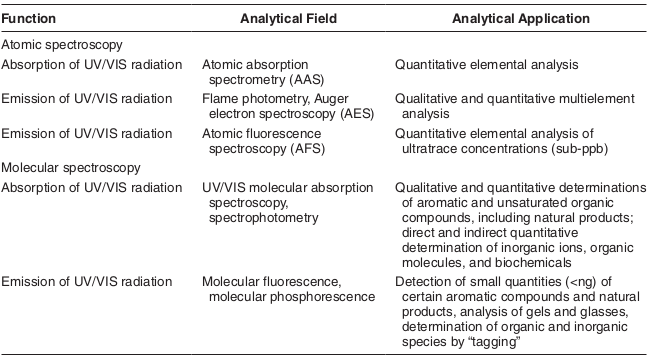
\includegraphics[width=0.9\textwidth]{2021-01-02_17-55.png}
\end{table}
紫外线和可见辐射与物质的相互作用可以定性地鉴定分子和多原子物质,包括离子和
络合物。可以获取有关分子和多原子物种(尤其是有机分子)的结构信息。该定性信息
通常是通过观察UV/VIS光谱,UV吸收和可见辐射随分子的波长而获得的。图\ref{fig:5.1}
(a)至(c)显示了某些有机化合物的典型紫外吸收光谱。光谱可以绘制成波长与吸光度,
透射率或摩尔吸收率$\varepsilon$的关系。随后定义摩尔吸光率。在图\ref{fig:5.1}中
,将溶解在乙醇中的吡啶的吸收光谱绘制为$\log\varepsilon$与波长(以埃为单位)的
关系。图\ref{fig:5.1}(b)和(c)绘制为吸光度与波长(nm)的关系。在这些光谱中看到
的较旧的波长单位为$\mu$m;该单位已被国际系统单位(SI)单位nm取代。注意
图\ref{fig:5.1}(b)和(c)中需要稀释。在图\ref{fig:5.1}(b)中,将溶液以1:10的比例
稀释,使峰在275 nm处成比例。在图\ref{fig:5.1}(c)中,浓度为0.140 g/L时,在230和
222 nm处的吸光度峰不合比例。将该溶液稀释至0.038 g/L的浓度,并在较小光程
的池中运行。

\begin{figure}[htpb]
    \centering
    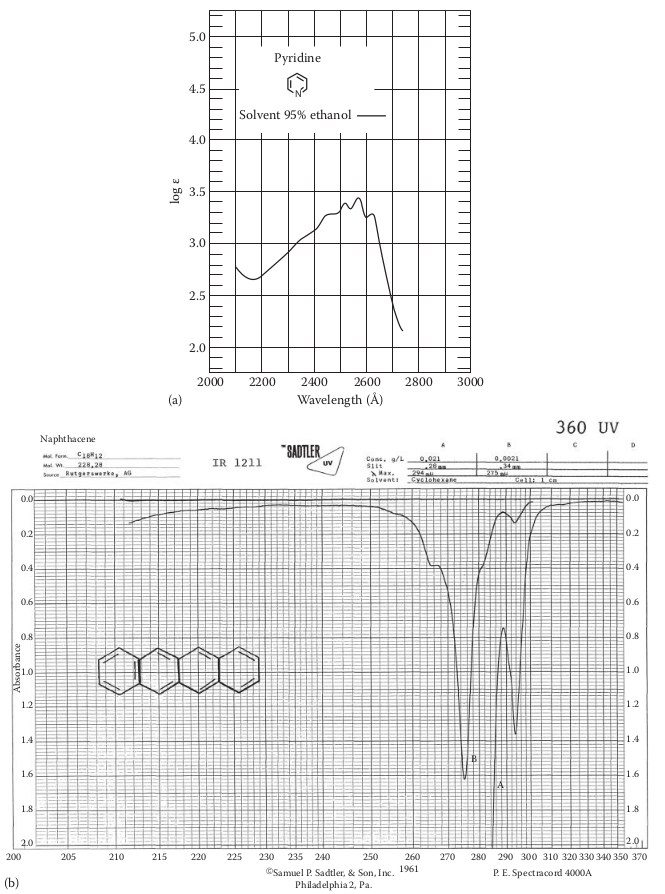
\includegraphics[width=0.95\textwidth]{2021-01-02_19-26.png}
\end{figure}
%\addtocounter{figure}{-1}
\begin{figure}[htpb]
    \centering
    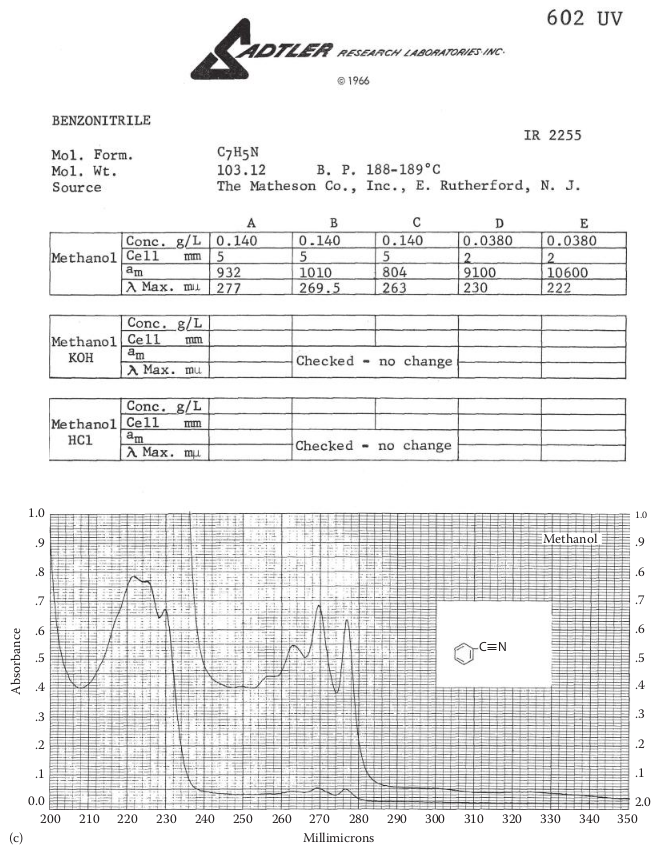
\includegraphics[width=0.95\textwidth]{2021-01-02_19-17.png}
    \caption{几种有机分子溶液的紫外吸收}
    \label{fig:5.1}
\end{figure}

还可以通过研究分子或多原子物质对紫外线和可见辐射的吸收或发射来获得定量信息。
作为一个非常简单的示例,我们可以查看红色溶液(例如红色墨水在水中)的吸收光谱
(图\ref{fig:5.2})。可以看出,对于无色纯净水样品(如虚线所示),所有波长的
白光(包括所有红色波长)都通过样品透射。如果我们向水中添加一滴红色墨水,使溶液
看起来呈浅红色,则光谱表明已吸收了部分蓝色和部分黄色的光,但已透射了所有红色
的光。如果我们在水中添加更多的红色墨水制成深红色溶液,则大部分蓝色和黄色光已被
吸收,但所有红色光都已透射。每种情况下,落在眼睛或检测器上的红光量都相同。溶液
中的墨水量与吸收的蓝光和黄光有关,与透射的颜色无关。我们可以在水中构造一系列
已知量的红色墨水,并通过测量在例如450 nm处吸收的光量来定量测量其他墨水溶液。
样品(尤其是溶液)中物种的浓度通常使用UV/VIS吸收光谱法或荧光光谱法进行测量。
浓度或浓度变化的测量可用于计算化学系统的平衡常数、反应动力学和化学计量。通过
UV/VIS光谱仪进行的定量测量在环境监控、食品和饮料制造等工业过程控制、药品质量
控制和临床化学等方面很重要。分子激发后,分子以多种方式发生辐射。荧光和磷光是
两个过程。
\begin{figure}[htpb]
    \centering
    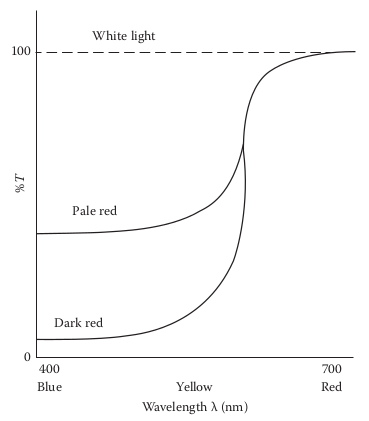
\includegraphics[width=0.6\textwidth]{2021-01-02_19-22.png}
    \caption{可见吸收示例}
    \label{fig:5.2}
\end{figure}
\subsection{分子中的电子激发}
分子由原子组成,这些原子通过共享电子而保持在一起,形成化学键。分子中的电子以
量子理论定义的离散能级在分子轨道中移动。当电子的能量最小时,分子处于最低能量
状态或基态。分子可以吸收辐射并移动到更高能量的状态或激发状态。当分子激发时,
外壳(价)电子移动到能量更高的轨道。将电子移动到更高能态的过程称为电子激发。
为了使辐射引起电子激发,它必须在电磁光谱的可见光或紫外线范围内。分子吸收或发射
的频率与辐射能量之间的关系是$\Delta E = h\nu$。所需的实际能量取决于电子的基态
$E_0$和激发态$E_1$之间的能量差。关系描述为
\begin{equation}
    \Delta E = E_1 - E_0 = h\nu
    \label{5.1}
\end{equation}
$E_1$是激发态能量;$E_0$是基态能量。
可能需要在常规化学教科书或参考书目中列出的Chang或Zumdahl的教科书中查看键合,
分子轨道,路易斯结构和有机化学的主题,以帮助您理解随后讨论的材料。讨论将集中在
有机分子上,因为键合相对容易理解。无机分子也像有机分子与金属离子的络合物一样
吸收和发射紫外线和可见光,但是由于d和f轨道中的电子,无机分子中的键合以及过渡
金属与较重元素的络合物也很复杂。

分子中的价电子跃迁涉及三种不同类型的电子。首先是涉及单键的电子,例如烷烃中碳
和氢之间的电子。这些键称为sigma($\sigma$)键。激发$\sigma$键中的电子所需的
能量通常大于200 nm的UV光子。因此,烷烃和其他饱和化合物(仅具有单键的
化合物)不吸收紫外线辐射,因此通常非常可用作研究其他分子的透明溶剂。这种
不吸收性化合物的一个例子是正己烷(\ce{C6H14})。

接下来,我们使电子参与双键和三键(不饱和键)。这些键包括一个$\pi$键。具有$\pi$
键的化合物的典型例子是烯烃,炔烃,共轭烯烃和芳族化合物(图\ref{fig:5.3})。
$\pi$键中的电子相对容易被激发。这些化合物通常在紫外线或可见光区域吸收。
\begin{figure}[htpb]
    \centering
    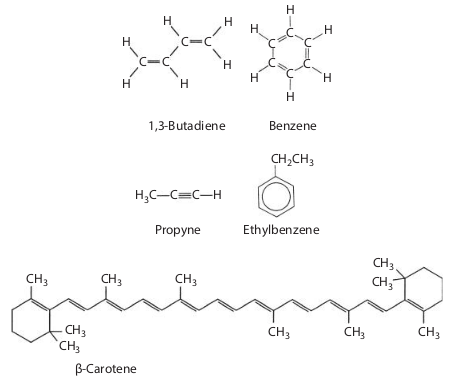
\includegraphics[width=0.75\textwidth]{2021-01-03_01-28.png}
    \caption{含$\pi$键有机物示例}
    \label{fig:5.3}
\end{figure}

原子间不参与原子键合的电子是分子中的第三类电子。对于非键合电子,这些被称为$n$
电子。在饱和烃中,碳和氢的外壳电子都参与键合;因此,这些化合物不具有任何$n$
电子。但是,含有氮,氧,硫或卤素的有机化合物通常含有不键合的电子(图
\ref{fig:5.4})。由于$n$电子通常被UV或可见光辐射激发,因此许多包含$n$电子的
化合物都会吸收UV/VIS辐射。
\begin{figure}[htpb]
    \centering
    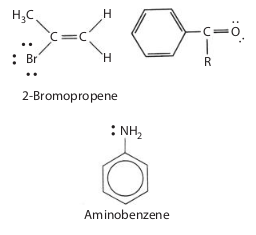
\includegraphics[width=0.5\textwidth]{2021-01-03_01-32.png}
    \caption{含非键有机物示例}
    \label{fig:5.4}
\end{figure}

图\ref{fig:5.5}中显示了在相邻原子上的原子轨道上的两个s电子结合形成$\sigma$键的
示意性能量图。轨道是守恒的;因此,形成两个分子轨道:
一个$\sigma$成键轨道和一个能量更高的$\sigma^\ast$反键轨道。$\sigma$和$\sigma
^\ast$之间的能量差等于$\Delta E$,如大箭头所示。每个原子都有三个2p原子轨道。
这些p轨道中的一个可以与相邻原子上的p轨道重叠,以形成第二组$\sigma$轨道。其他
两个p轨道可能会发生侧向重叠,形成$\pi$成键和$\pi^\ast$反键轨道。形成一组$\pi$
轨道的示意性能量图如图\ref{fig:5.6}所示,大箭头显示了$\pi$成键轨道和$\pi^\ast$
反键轨道之间的能量差。如果p轨道充满一对电子,它将不会形成键。图\ref{fig:5.7}
显示了一个填充的原子p轨道(在右边的原子中)可以形成一个非键合$n$轨道,该能量
不会从原子轨道上转移出来,而每个原子上部分填充的p轨道重叠形成一对
$\pi$键和$\pi^\ast$键轨道。
\begin{figure}[htpb]
    \centering
    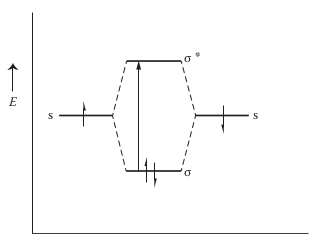
\includegraphics[width=0.5\textwidth]{2021-01-03_01-35.png}
    \caption{两个s原子轨道形成$\sigma$成键和$\sigma^\ast$反键分子轨道}
    \label{fig:5.5}
\end{figure}
\begin{figure}[htpb]
    \centering
    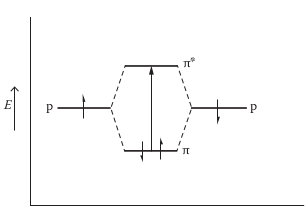
\includegraphics[width=0.5\textwidth]{2021-01-03_01-54.png}
    \caption{两个p原子轨道形成$\pi$成键和$\pi^\ast$反键分子轨道}
    \label{fig:5.6}
\end{figure}
\begin{figure}[htpb]
    \centering
    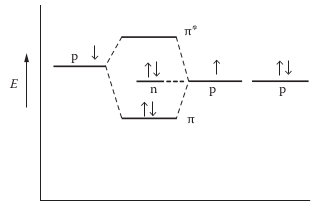
\includegraphics[width=0.5\textwidth]{2021-01-03_01-53.png}
    \caption{p原子轨道形成$\pi$成键、$\pi^\ast$反键和非键$n$分子轨道}
    \label{fig:5.7}
\end{figure}

$\sigma$、$\pi$和$n$电子的相对能图如图\ref{fig:5.8}所示,但该一般顺序有例外。
可以看出,将电子从$\sigma$激发到$\sigma^\ast$轨道所需的能量远大于将电子从
$\pi$激发到$\pi^\ast$轨道,或将$n$电子激发到$\sigma^\ast$或$\pi$所需的能量。
结果,将$\sigma$电子激发到$\sigma^\ast$轨道所需的能量大于在UV区域中可用的能量,
但是通常UV辐射足以将$\pi$轨道中的电子激发到$\pi^\ast$反键轨道,
或将$n$个电子激发到$\pi^\ast$或$\sigma^\ast$。
\begin{figure}[htpb]
    \centering
    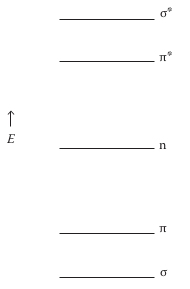
\includegraphics[width=0.25\textwidth]{2021-01-03_01-58.png}
    \caption{$\sigma$成键、$\sigma^\ast$反键、$\pi$成键、$\pi^\ast$反键和非键
    $n$分子轨道能级示意图}
    \label{fig:5.8}
\end{figure}
\subsection{分子吸收}
量子力学为理解分子轨道的相对能级,以及它们如何随结构变化提供理论基础。量子力学
还生成一组“选择规则”,以预测分子中发生的跃迁。分子中发生的跃迁受这些量子力学
选择规则支配。选择规则“允许”某些转换,而“禁止”进行其他转换。选择规则超出本文的
范围,但可以在大多数物理化学文章中或在参考书目中列出的Ingle和Crouch的文章中
找到。与规则一样,也有例外,并且确实发生许多禁止的过渡,并且
可以在UV/VIS光谱中看到。

当分子被电子激发时,电子从占据最高的分子轨道移动到最低的未占据的轨道,该轨道
通常是反键轨道。$\pi$键中的电子被激发成反键$\pi^\ast$轨道,$n$个电子被激发到
$\sigma^\ast$或$\pi^\ast$轨道。

有机分子和无机分子都可能表现出UV/VIS辐射的吸收和发射。吸收可见光或紫外线的
分子基团称为生色团,在希腊语中称为色度(chromophores)。例如,为了发生
$\pi\to\pi^\ast$跃迁,分子必须具有带有不饱和键(例如C$=$C, C$=$O和
C$=$N)的发色团。具有这些类型的生色团的化合物包括烯烃,酰胺,酮,羧酸和肟
等。通常在UV/VIS区域发生的另一种过渡是$n\to\pi^\ast$过渡,因此包含具有未键合
电子的原子的有机分子应能够吸收UV/VIS辐射。这样的原子包括氮,氧,硫和卤素原子,
尤其是Br和I。表\ref{tab:5.2}列出了一些用作生色团的典型有机官能团。表
\ref{tab:5.3}列出了有机化合物的类型及其最大吸收波长,即吸收最多光的波长。一些
化合物具有一个以上的吸收峰,因此列出了多个“最大值”。诸如烷烃之类的化合物仅包含
$\sigma$键,它们不吸收可见光或UV区域的辐射。
\begin{table}[htbp]
    \centering
    \caption{UV/VIS下有吸收的有机官能团}
    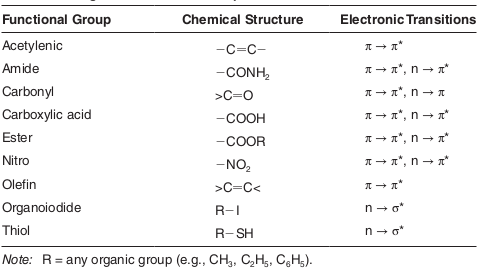
\includegraphics[width=0.7\textwidth]{2021-01-03_09-35.png}
    \label{tab:5.2}
\end{table}
\begin{table}[htbp]
    \centering
    \caption{典型有机官能团最大吸收波长}
    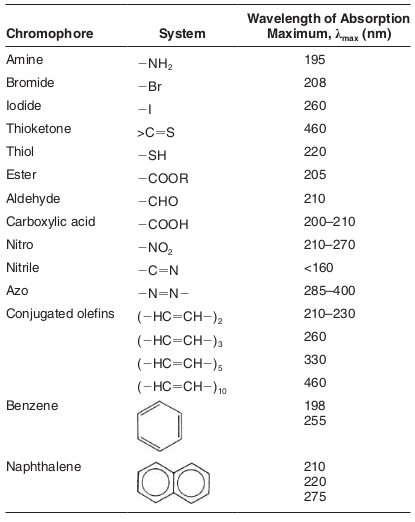
\includegraphics[width=0.6\textwidth]{2021-01-03_09-36.png}
    \label{tab:5.3}
\end{table}

过渡金属化合物通常是有色的,表明它们吸收光谱可见部分的光。这是由于存在未填满的
d轨道。吸收带最大值的确切波长取决于d轨道电子的数量,化合物的几何形状以及与
过渡金属配位的原子。
\subsection{摩尔吸光系数}
上一章我们介绍涉及光程和样品浓度的Beer定律,其中,$\varepsilon$为摩尔吸光系数。
为给定波长、给定浓度下,所吸收的辐射。
\begin{equation}
    A = \varepsilon l c
    \label{5.2}
\end{equation}
浓度$c$的单位是mol$\cdot$L$^{-1}$,光程$l$的单位是cm,那么,$\varepsilon$的单位
为L$\cdot$mol$^{-1}\cdot$cm$^{-1}$。通常,$\varepsilon\approx 10^4 - 10^5$ 
范围的跃迁是允许的,10--100范围内的跃迁,是禁阻的。较高的$\varepsilon$值,对
特定波长的光,有强吸收;较低值,对应弱吸收。$\varepsilon$表明特定波长下,分子
的物理性质。最大吸收波长的符号为$\lambda_{max}$,同理,最大的摩尔吸光系数表示
为$\varepsilon_{max}$。表\ref{tab:5.4}列出一些常见有机分子$\lambda_{max}$和
$\varepsilon_{max}$的典型值。
\begin{table}[htbp]
    \centering
    \caption{常见发色团典型的最大吸收峰和摩尔吸光系数}
    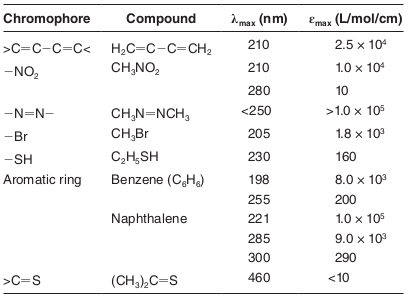
\includegraphics[width=0.6\textwidth]{2021-01-04_20-57.png}
    \label{tab:5.4}
\end{table}

测量吸收的波长范围比吸收带宽要窄,所以摩尔吸光系数不能直接衡量电子跃迁的可能性
。摩尔吸光系数,在整个波段范围内的不同波长处,是不相同的。有几个与跃迁概率
直接相关的基本量,如爱因斯坦系数和振荡器强度$f$。
\subsection{紫外吸收曲线形状}
图\ref{fig:5.1}是溶液中有机分子典型的紫外吸收光谱。每个光谱看起来非常简单,
在很宽的波长范围内,具有较宽的吸收“带”,而不是在红外(IR)光谱中看到的众多的
较窄的吸收峰。分子中每个电子的能级都有与其相关的多个振动和转动能级,导致吸收带
非常宽。电子从基态到激发态的跃迁,所达到的不止一个激发态的振动和转动能级。
电子跃迁振动和转动能级示意图如图\ref{fig:5.9}所示。在基态,仅显示最低的振动
能级,带有四个转动子能级。室温下,多数分子处于最低振动状态的基态。激发态中,
显示四个振动子能级,每个振动能级里,有差别很小的转动子能级。在许多可能的跃迁
类型中,选取四种显示在图中;每一个箭头对应一个吸收波长。电子跃迁是有大量波长
组成连续的吸收带。尽管每一个跃迁是量子化的,靠近振动能级,或者,靠近转动能级的
能量空间,导致电子跃迁是一个带光谱。如图\ref{fig:5.10}所示。
\begin{figure}[htpb]
    \centering
    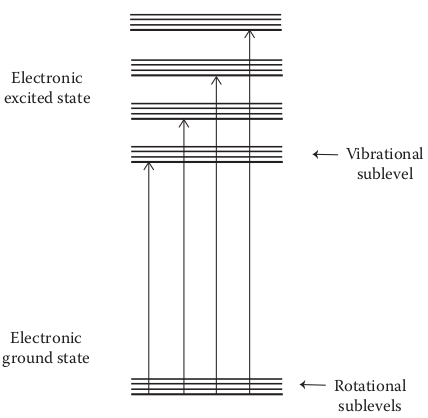
\includegraphics[width=0.55\textwidth]{2021-01-08_20-45.png}
    \caption{电子跃迁能量带源于电子具有多个振动和转动能级}
    \label{fig:5.9}
\end{figure}
\begin{figure}[htpb]
    \centering
    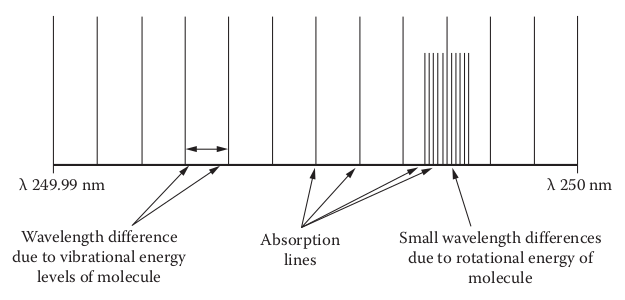
\includegraphics[width=0.85\textwidth]{2021-01-08_20-48.png}
    \caption{UV吸收带}
    \label{fig:5.10}
\end{figure}

吸收带的特征在于其形状,即其宽度和强度。带的形状主要由振动能级间隔和每个振动
跃迁的强度决定。强度分布与跃迁到给定振动能级的可能性有关。跃迁概率可以使用
弗兰克-康登(Franck-Condon)原理确定。 参见Hollas和Lambert等人的文章。可以说,
如果我们有一百万个分子,即使它们在激发前大多处于基态振动状态,但在激发后它们
可能处于各种振动状态。引起电子激发到每个振动能级所需的辐射能略有不同,并且会
通过转动能的变化进一步改变。因此,当紫外辐射落在这一百万个分子上时,它会在许多
波长处被吸收。吸收波长的总范围可能会延长至100 nm范围内。分子转动能级,使得吸收
线更加变成单一的吸收带。吸收线数目的增加,使得线彼此接近,但不会增加吸收带的
总宽度。这是因为引入的转动能级与振动能级相比,很小,与电子跃迁相比,就更小了。
因此,紫外辐射是吸收带,而不是离散的波长。

在许多实际测试中,UV/VIS光谱显示了不同的振动能级。例如,气相中简单的分子的振动
跃迁,经常与电子跃迁叠加在一起,如图\ref{fig:5.11}所示气相苯的吸收光谱。宽
谱带顶部的尖峰,是振动能级的“精细结构”。溶液中的分子(如图\ref{fig:5.1})通常
不具备这种振动结构,是由于溶剂和溶质分子间的相互作用导致的。相比于气相苯的吸收
,溶液中苯的吸收光谱(如图\ref{fig:5.12}),大多数的精细结构消失不见。可见,
精细结构源于转动能级,在常规的UV/VIS中,无法观察到;商业仪器没有这么高的解析度
,可以观察到这些线。
\begin{figure}[htpb]
    \centering
    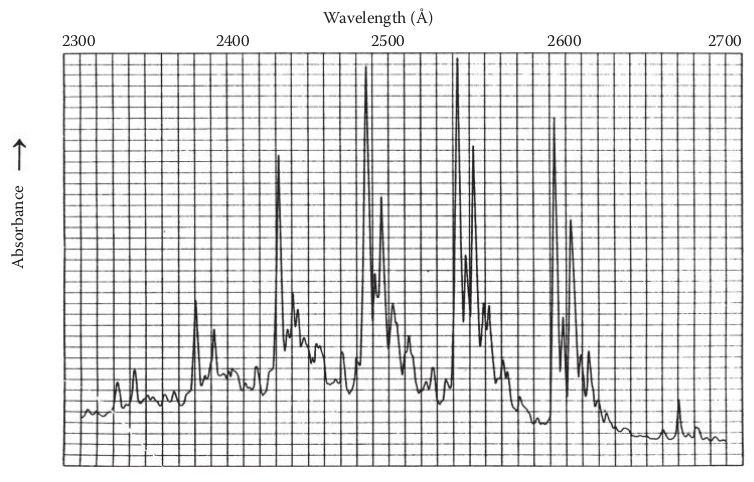
\includegraphics[width=0.85\textwidth]{2021-01-08_22-16.png}
    \caption{气相苯的吸收光谱}
    \label{fig:5.11}
\end{figure}
\begin{figure}[htpb]
    \centering
    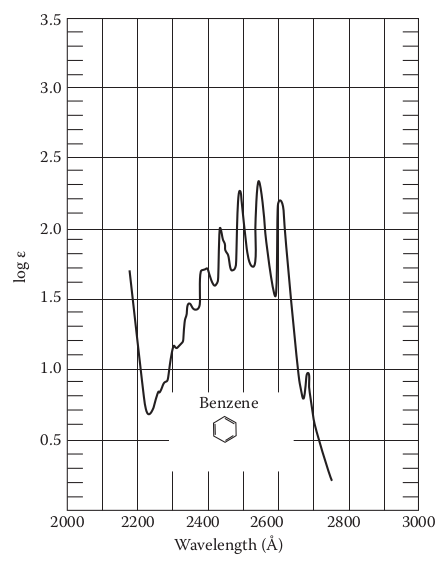
\includegraphics[width=0.55\textwidth]{2021-01-08_22-18.png}
    \caption{溶液中苯的吸收光谱}
    \label{fig:5.12}
\end{figure}
\subsection{UV/VIS光谱的溶剂}
绝大多数的吸收光谱是在溶液中测量的。溶质必须可溶于溶剂,并且溶剂必须在目标
波长范围内是透明的(无吸收)。形成溶液的使能量降低。溶质和溶剂之间的分子间
吸引力必须大于溶质-溶质和溶剂-溶剂之间的吸引力。溶液形成所涉及的力是偶极-偶极
吸引,氢键和范德华力。极性起着主要作用,并产生了“like dissolves like”的规则。
与非极性溶剂相比,极性物质在极性溶剂中的溶解更容易。溶质要完全溶解是很重要的。
未溶解的粒子会散射来自光源的光。这可能会导致定性和定量分析中的严重误差。

溶剂有时会严重影响光谱的形状。极性溶剂通常会消除光谱中的振动精细结构。溶剂也会
移动吸收带的位置。对于光谱的可见区域,可以使用样品可溶于其中的任何无色溶剂。

UV/VIS光谱学中使用的常见溶剂及其低波长截止值列于表\ref{tab:5.5}中。在比截止
波长短的波长处,溶剂吸收太强而无法在标准的1 cm样品池中使用。临界值受溶剂纯度
的影响。对于光谱学,溶剂应属于光谱或光谱化学级,符合美国化学学会规定的纯度要求。
\begin{table}[htbp]
    \centering
    \caption{常用紫外光谱测试的溶剂及其截止波长}
    \label{tab:5.5}
    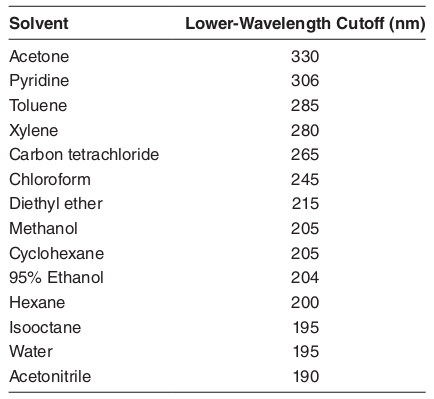
\includegraphics[width=0.5\textwidth]{2021-01-08_22-37.png}
\end{table}
\section{仪器}
\subsection{光学系统}
光谱仪是测量吸收或透过的光的强度,并作为波长的函数的仪器设备。单光束或双光束
用于分子吸收光谱的测量。单光束系统和它的三个缺点,已经在上一章讨论过。绝大多数
商业仪器都使用双光束系统,我们重点讨论一下。

双光束系统将辐射源分成强度相等的两份光路。两束光穿过两条长度相同的光路;
\emph{参比}池放在一个路径中,而\emph{样品}池则在另一路径中。然后比较穿过两池的
两个光束的强度。由于功率波动,光学系统损失的辐射(例如,样品池表面和反射镜,
溶剂吸收的辐射等),导致辐射强度变化对于两个光束都应相等,以校正这些误差源。
用于吸收光谱的色散光谱仪被称为分光光度计,该色散光谱仪具有一个或多个出口狭缝和
光电检测器,该光电检测器将两个光束的强度与波长成比例。

商用UV/VIS光谱仪设计为在200--800 nm范围内的空气中与空气一起运行。用干燥的氮气
吹扫光谱仪可以观察到低至175 nm的波长。如前所述,对于较低的波长,必须将光谱仪
置于真空下或用不吸收气体吹扫。在分析上,由于需要真空的仪器固有的困难和费用,
真空紫外线区域对常规分析的重要性不高。

使用滤光片进行波长选择和光电检测器的简单光学系统称为光度计。光度计用于可见光
区域和紫外线区域。例如,紫外光度计通常用作高效液相色谱(HPLC)中的检测器,但已
被光电二极管阵列(PDA)取代。 HPLC检测器将在后续章节中详细讨论。

所有用于吸收测量的光谱仪都需要一个光源,一个波长选择设备,一个样品架和一个
检测器。可以从许多商业仪器公司获得完整的UV/VIS和UV/VIS/近红外(NIR)系统,包括
安捷伦科技公司,PerkinElmer,Shimadzu Scientific Instruments和Thermo Fisher 
Scientific。这些大型公司各自提供具有不同功能的5至8个版本的系统。他们的网站提供
应用程序,有关使用仪器的视频,教程以及许多其他有用的信息。
\subsection{辐射源}
用于分子吸收测量的辐射源必须产生连续波长的光。理想地,光源的强度在所有发射的
波长上将是恒定的。传统上,用于UV/VIS光谱的两个最常见的辐射源是钨灯和氘灯。钨灯
的功能类似于普通的白炽灯泡。它包含一个钨丝,该钨丝被电加热至白热并产生连续
光谱。它有两个缺点:短波长($<$ 350 nm)的辐射强度低;此外,为了保持恒定的强度,
必须小心地控制灯电流。但是,这些灯通常是稳定,坚固且易于使用的。发射强度随波长
变化,如图\ref{fig:5.13}所示。这些曲线的形状是加热到白炽灯的固体连续输出的典型
特征。产生这种曲线的白炽体称为黑体辐射器。连续发射是由于固体(在这种情况下是
钨丝)中的热激发跃迁引起的。黑体辐射器的强度与波长的关系图取决于发射材料的温度
,而不取决于其化学成分。钨灯在可见光范围内最有用,通常在分光光度法中使用,随后
进行讨论。由于仅在可见光区域使用灯泡,因此灯泡可以由玻璃而不是石英制成。紫外光
的传输需要石英。与现代汽车前照灯中的灯类似,钨卤素灯已取代了现代仪器中较旧的
钨灯。钨卤素灯有一个石英灯泡,主要用来承受灯的高工作温度。该灯比钨灯高效得多,
并且使用寿命更长。钨卤素灯的波长/强度输出如图\ref{fig:5.14}所示。
\begin{figure}[htpb]
    \centering
    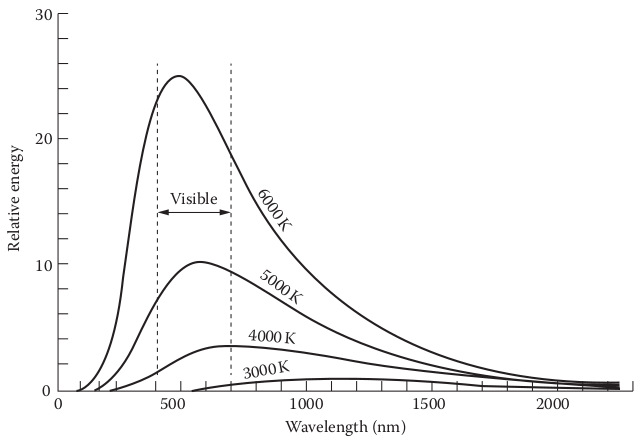
\includegraphics[width=0.75\textwidth]{2021-01-09_10-11.png}
    \caption{黑体辐射的发射强度}
    \label{fig:5.13}
\end{figure}
\begin{figure}[htpb]
    \centering
    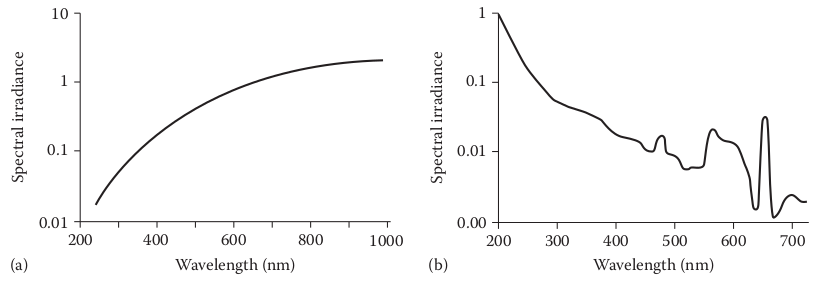
\includegraphics[width=0.85\textwidth]{2021-01-09_10-13.png}
    \caption{(a)商用钨卤灯发射光谱;(b)商用氘弧灯发射光谱}
    \label{fig:5.14}
\end{figure}

\emph{氘弧灯}由石英灯泡中的氘气(\ce{D2})组成,放电时通过氘气。分子被电激发,
被激发的氘分子解离,发出紫外线。氘分子解离成原子会导致在从0到分子激发能的连续
能量范围内发出UV光子。这会导致灯在160--400 nm的范围内发出连续的(宽带)UV光谱,
而不是窄线原子发射光谱。该灯稳定,坚固并且被广泛使用。使用氘代替氢气的效果是,
在UV范围的短波长端发射强度增加多达三倍。虽然氘比氢更昂贵,但获得所需的高强度
的光源。图\ref{fig:5.14}(b)给出了氘弧灯的发射光谱。

\emph{氙弧灯}的工作方式类似于氘灯。氙气通过电流会在200--1000 nm范围内产生强烈
的辐射。它们提供非常高的辐射强度,并且它们不需要预热时间,因此被广泛用于现代
UV/VIS仪器中。该灯用于荧光光谱法,其灯的原理图和光谱见后续章节。如今,许多
UV/VIS光谱仪都使用氙气闪光灯,氙气闪光灯仅在读取读数时才会闪烁。它们不需要预热
时间,并且只需很少的电能。用这种类型的灯可以消除光降解,因为样品不会暴露在大量
的辐射或热量下。

最近引入的重要光源是发光二极管(LED)。 LED由掺有杂质的半导体材料芯片组成,以
形成PN结(见图\ref{fig:5.21})。电流从阳极的p侧流向阴极的n侧。电荷载流子,电子
和空穴从具有不同电压的电极流入结中。当电子遇到空穴时,它会降到较低的能级并发射
光子。发出的光的波长(其颜色)取决于形成PN结的材料的带隙能量(图
\ref{fig:5.15}(a)和\ref{fig:5.20})。 LED原理图如图\ref{fig:5.15}(b)所示。
\begin{figure}[htpb]
    \centering
    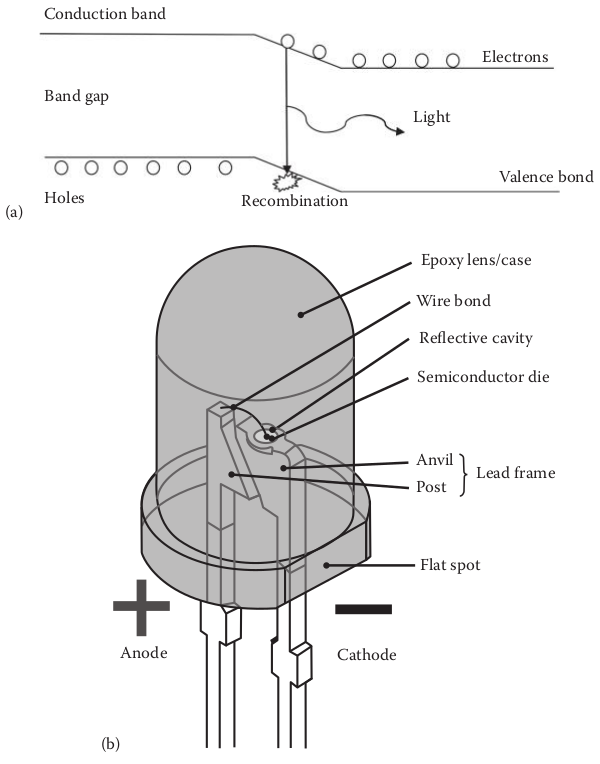
\includegraphics[width=0.75\textwidth]{2021-01-09_11-55.png}
    \caption{(a)LED中电子和空穴;(b)LED构造}
    \label{fig:5.15}
\end{figure}

现在,可以使用各种可见颜色的商用LED以及发射IR和UV的LED。发出紫外线的LED通常由
氮化硼(\ce{BN}),氮化铝(\ce{AlN}),氮化铝镓(\ce{AlGaN})和氮化铝镓铟
(\ce{AlGaInN})制成。为了创建用于可见光谱的白光源,使用了两种方法。一种是将
红色,绿色和蓝色LED混合使用以产生白光。红色LED是第一个实际应用的LED,也是第
一个商业化的LED,它由磷化镓(\ce{GaP}),砷化镓磷化物(\ce{GaAsP}),砷化铝镓
(\ce{AlGaAs})和磷化铝镓铟磷(\ce{AlGaInP})制成。绿色LED基于氮化铟镓
(\ce{InGaN}),磷化铝镓(\ce{AlGaP})和类似材料。蓝色LED由氮化铟镓
(\ce{InGaN}),硒化锌(\ce{ZnSe})和其他材料制成。第二种方法是在开发高强度
蓝色LED之后实用的,它是使用蓝色LED和基于氧化钇铝(也称为YAG)等材料的荧光粉
涂层。磷光体产生的黄光与蓝光结合时会变成白色,这与标准荧光灯泡的工作方式
非常相似。
\subsection{单色器}
单色器的目的是根据波长分散辐射,并允许选定的波长照亮样品。衍射光栅用于在现代
仪器中散射光,如前所述。现代系统中的单色器,例如安捷伦科技公司的Cary分光光度计
,可以以高达2000--3000 nm/min的速率扫描,并具有摆率(在不进行测量的情况下,
在波长之间移动的时间)高达16000 nm/min,以适应制药和生物技术实验室所需的
高通量测量。

新的衍射光栅技术允许进行几年前无法进行的测量。由离子束或激光束光刻技术产生
的前一章中讨论的衍射光栅,由于表面粗糙度,会产生杂散光(不需要的波长的光)。
如今,为优化与全息技术一起使用的蚀刻工艺而开发的新型专有制造方法可大大改善
衍射光栅,例如Shimadzu Scientific Instruments(www.ssi.shimadzu.com)的
“Lo-Ray-Ligh”光栅。Lo-Ray-Ligh光栅具有低至0.00005 \%的超低杂散光值,可在高达
8.5吸光度单位的情况下以完全线性的方式进行吸光度测量。图\ref{fig:5.16}(a)比较了
使用Lo-Ray-Ligh光栅在UV-2700上获得的吸收光谱与在常规光谱仪上获得的吸收光谱。
图\ref{fig:5.16}(b)展示了超过8.5个吸光度单位的线性。这样可以测量高吸收性材料,
例如太阳镜偏光镜和焊接面罩。在下一节中将给出一些示例。
\begin{figure}[htpb]
    \centering
    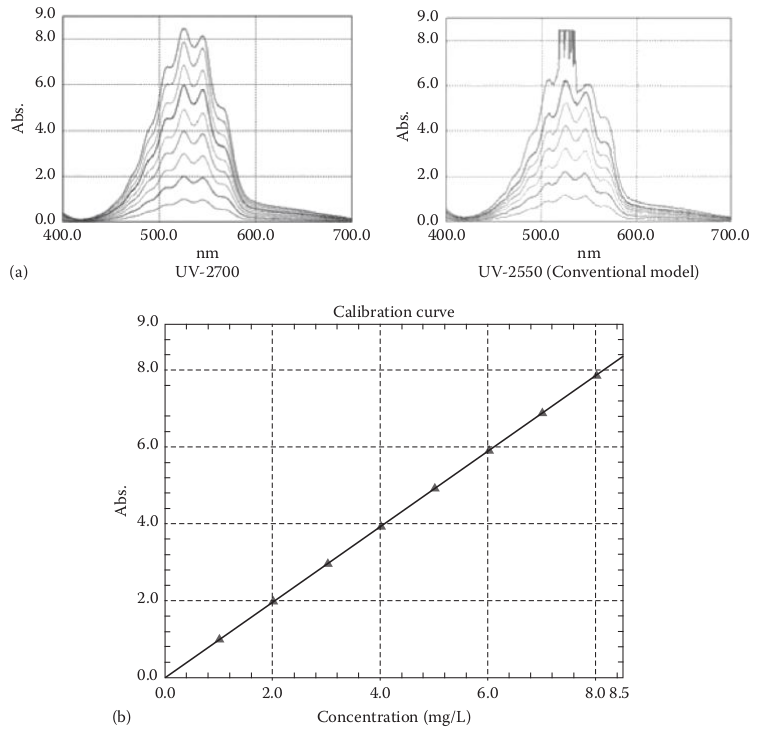
\includegraphics[width=0.85\textwidth]{2021-01-09_12-14.png}
    \caption{(a)左:使用Lo-Ray-Ligh光栅的UV-2700光谱仪获得的光谱;右:常规光谱
    仪获得的光谱(超出范围)(b)UV-2700校正曲线,吸光度为8.5依然保持线性}
    \label{fig:5.16}
\end{figure}
\subsection{检测器}
最早用于可见光谱的检测器是人眼。仍然有专为视觉观察颜色和强度而设计的分光镜和
颜色比较器。

大多数现代仪器都依赖于{\bf 光电转换器},将光子转换成电信号的检测设备。光电转换
器的表面可以吸收辐射能。吸收的能量要么导致电子发射,从而产生光电流,要么将电子
移动到固体半导体的导带中,从而导致电导率增加。这些检测器有几种常见形式,包括
势垒层电池、光电倍增管(PMT)和半导体检测器。
\subsubsection{势垒层电池}
在势垒层电池(也称为光伏电池)中,吸收辐射后会在金属和半导体的界面处产生电流。
例如,将银涂在半导体(例如硒)上(参见图\ref{fig:5.17}),该半导体与诸如铁之类
的坚固金属基体相连。为了制造这些电池,将硒放入容器中,并将气压降低至真空。银被
电加热,其表面熔化和汽化。银蒸气覆盖硒表面,形成非常薄但均匀分布的银原子层。
落在表面上的任何辐射都会在硒-银界面处产生电子和空穴。硒和铁之间似乎存在一个
屏障,可以阻止电子流入铁中。电子流向银层,空穴流向铁。电子被银收集。这些收集的
电子通过外部电路向空穴迁移。以这种方式产生的光电流与撞击的光子数量成正比。
\begin{figure}[htpb]
    \centering
    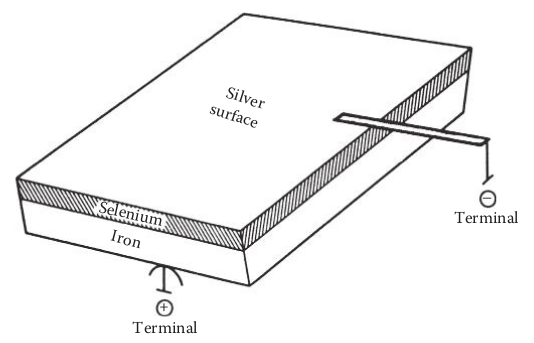
\includegraphics[width=0.65\textwidth]{2021-01-09_12-34.png}
    \caption{势垒层电池}
    \label{fig:5.17}
\end{figure}

势垒层电池在照相机和低成本便携式仪器中用作检测器。响应范围是350--750 nm。这些
检测器有两个主要缺点:它们在弱光下不灵敏并且显示出\emph{疲劳感},也就是说,
在持续暴露
于光线下电流会逐渐下降。从好的方面来说,它们不需要外部电源,并且非常坚固。
\subsubsection{光电倍增管}
PMT是一种非常常见的检测器。 PMT是密封的,抽空的透明外壳(石英或玻璃),包含
光电发射阴极、阳极和几个称为倍增极的其他电极。光电发射阴极是涂有碱金属或元素
混合物(例如Na/K/Cs/Sb或Ga/As)的金属,当被光子撞击时会发射电子。 PMT是真空
光电管的更复杂的版本,图\ref{fig:5.18}(a),其中仅包含光电发射阴极和阳极。
光电流仅限于从阴极发射的电子。在PMT中,图\ref{fig:5.18}(b)中,额外的倍增极将
可用电子“相乘”。喷射的电子被吸引到倍增极,该倍增极相对于阴极保持在正电压。到达
倍增极后,每个电子都会撞击倍增极的表面,并使表面再发射出几个电子。这些发射的
电子又被第二倍增极所吸引,在第二倍增极中,类似的电子发射和更多的倍增发生。重复
该过程数次,直到大量电子到达阳极(即集电极)为止。落在收集器上的电子数量是落在
检测器上的光强度的量度。在此过程中,单个光子可能会产生许多电子并发出高信号。
因此,倍增极工作在提供稳定信号的最佳电压下。商业PMT可能有九个或更多倍增极。
每个光子的增益可能高达$10^9$个电子。探测器系统的噪声水平最终会限制增益。例如,
增加倍增极之间的电压会增加信号,但是如果电压太高,来自检测器的信号就会变得
不稳定或嘈杂。在实践中,较低的增益和较低的噪声水平可能是更可取的。
\begin{figure}[htpb]
    \centering
    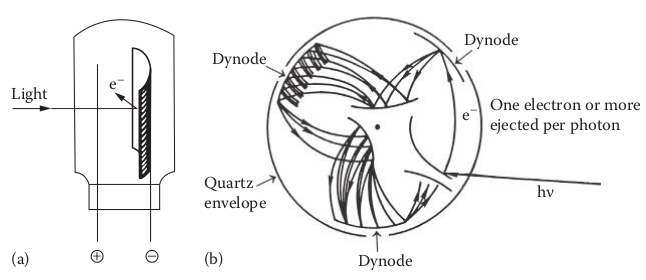
\includegraphics[width=0.75\textwidth]{2021-01-09_12-39.png}
    \caption{(a)真空光电管;(b)PMT构造图(俯视)}
    \label{fig:5.18}
\end{figure}

PMT对紫外线和可见辐射极为敏感。实际上,它们是如此敏感,以至于必须注意不要将
PMT暴露在强光下,以免造成损坏。有各种各样的光发射表面可用,它们可以响应不同的
波长范围。检测器信号与波长的关系曲线称为响应曲线。图\ref{fig:5.19}显示了商用
PMT的一些响应曲线。选择PMT检测器,以使其对目标波长范围具有最大响应。例如,IP28
在800 nm处不可用,但R136和Ga/As PMT检测器在此范围内有响应。PMT的响应时间非常快
,但是它们的暗电流限制了它们的灵敏度。暗电流是没有辐射落在检测器时,检测器发出
的恒定小信号。可以通过冷却检测器外壳来最小化或消除暗电流。为此目的,商业上
可加入冷却装置。
\begin{figure}[htpb]
    \centering
    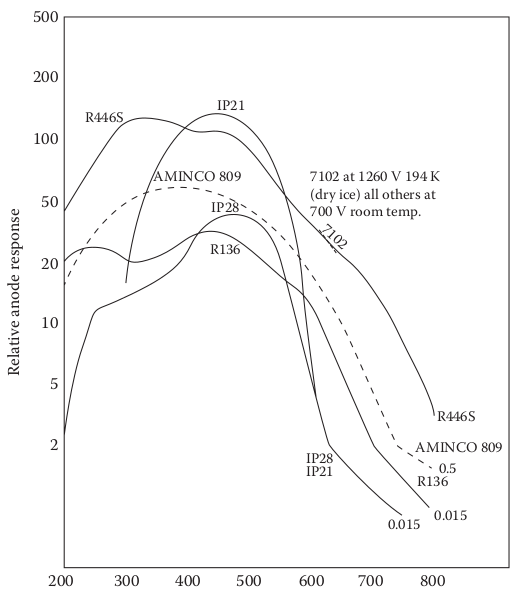
\includegraphics[width=0.65\textwidth]{2021-01-09_12-40.png}
    \caption{商用PMT响应曲线}
    \label{fig:5.19}
\end{figure}
\subsubsection{半导体检测器:二极管和二极管阵列}
固态半导体材料在电子设备和仪器中非常重要,包括用作辐射探测器。为了理解半导体
的行为,有必要简要描述这些材料中的键合。

当大量原子键合形成固体(例如固体硅)时,单个原子中存在的离散能级会扩散到固体中
的能带中。价电子不再局限于空间中的给定原子。能带的宽度随着固体中原子间间距的
减小而增加。至少部分被电子占据的最高能带称为价带;价带正上方的能带称为导带。
价带和导带被一个禁能范围隔开(量子力学禁止)。这种分离的幅度称为带隙,如图
\ref{fig:5.20}示意性地显示了一组能带和带隙。如果固体的价带在0 K的温度下完全
充满,则该材料是{\bf 半导体}或{\bf 绝缘体}。半导体和绝缘体之间的差异由带隙的
大小定义。如果$E_g \leq 2.5 \text{ eV}$,则该材料为半导体;如果$E_g >2.5$ eV,
则该材料为绝缘体。第三类材料,导体,在0 K处具有部分填充的价带。
\begin{figure}[htpb]
    \centering
    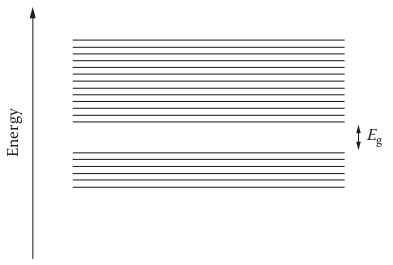
\includegraphics[width=0.65\textwidth]{2021-01-09_17-49.png}
    \caption{固体材料价带,$E_g$为带隙}
    \label{fig:5.20}
\end{figure}

半导体器件中最常使用的两个元素是硅和锗。两者均以固态共价键合且均属于元素周期表
的第IVA族。(在新的国际纯粹与应用化学联合会(IUPAC)术语中,该组也称为第14族,
在某些文本中,该组也称为IVA。)其他半导体包括\ce{GaAs},\ce{CdTe},\ce{InP}
以及其他无机和有机化合物。大多数半导体是共价键结合的固体。CRC的化学和物理手册中
列出了半导体的带隙能。

硅具有价电子结构\ce{3s^2{}3p^2}。部分填充的p轨道可能会导致人们假设硅具有部分填充
的价带,因此将成为导电体。因为硅是共价键合的,所以两个3s电子和两个3p电子占据了
\ce{sp^3}杂化轨道。这产生具有两个电子能带的固体,每个能带具有四个紧密间隔的子
能级,每个电子能带位于\ce{Si}的价电子壳中。四个电子占据并填充了0 K的价带,
因此不导电。但是,在高于0 K的温度下,一些电子会从价带热传导到导带;在那里,
它们成为电的导体。当电子离开价带时,它会留在也可以移动的正空穴之后,从而产生
一个电子-空穴对。电子和空穴都是半导体中的电荷载流子。诸如\ce{Si}和\ce{Ge}之类
的半导体称为本征半导体。它们的行为是纯材料的带隙和能带结构的结果。

可以通过向这些元素之一掺杂VA族元素(如砷或锑)或IIIA族元素(如铟或镓)来提高
电导率。掺杂是指向基质材料中添加其他物质。添加的物质称为掺杂剂。与掺杂原子关联
的电子与主体的能级不同,并且可能处在主体禁止的能级上。由添加掺杂剂引起的电导率
称为外在导电。VA族元素具有额外的电子(或额外的负电荷)。该电子不像主体的共价
键合电子那样牢固地保持,并且需要更少的能量才能将其移动到导带中。这是n型半导体。
类似地,添加IIIA组元素会导致电子“丢失”;这可以认为是产生了额外的正空穴。来自
掺杂剂原子的这些正空穴可以接受来自价带的电子。将电子移动到受体孔中所需的能量
小于将电子移动到导带中所需的能量。这是p型半导体。在n型半导体中,电子是可移动的
,而在p型半导体中,空穴是可移动的。在本征半导体中,每个激发事件都会形成两个电荷
载流子。在n型或p型非本征半导体中,每个激发事件仅形成一个电荷载流子。

半导体可用作电磁辐射检测器。$ E> E_g$的光子足以在半导体中创建其他电荷载流子。
额外的电荷载体会增加半导体的导电性。通过测量电导率,可以计算出光的强度。选择
具有合适带隙的材料可以在光谱的UV,可见光和IR区域产生光检测器。
\subsubsection{二极管}
二极管或整流器是一种电子设备,仅允许电流在一个方向上流动。如果我们将一个p型
半导体和一个n型半导体放在一起,那么这两种类型之间的结就是一个p–n结,如图
\ref{fig:5.21}所示。它由单片半导体通过将一侧掺杂为p型而另一侧掺杂为n型半导体
而形成。在两种类型相遇的地方形成连接点。在向器件施加任何电势之前,空穴将成为
p侧的主要电荷载流子,而电子将成为n侧的主要电荷载流子。如果我们在p型侧施加
正电势,而在n型侧施加负电势,如图\ref{fig:5.22}所示,则正电荷(空穴)从p区域
流向结,而负电荷从n型区域流向结。在结处或附近,空穴和电子复合并被猝灭。这称为
正向偏置,在这种情况下,电流容易流过半导体。电子-空穴对猝灭产生能量。如果这种
能量以光的形式出现,那么我们有前面讨论过的LED。
\begin{figure}[htpb]
    \centering
    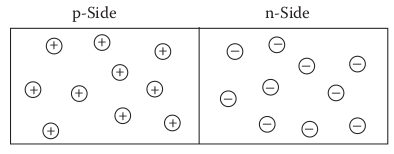
\includegraphics[width=0.55\textwidth]{2021-01-09_18-16.png}
    \caption{没有电势的p-n结}
    \label{fig:5.21}
\end{figure}
\begin{figure}[htpb]
    \centering
    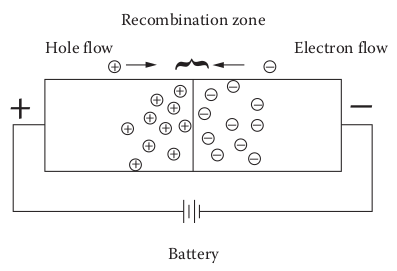
\includegraphics[width=0.55\textwidth]{2021-01-09_18-18.png}
    \caption{向前偏置的p-n结,电池的正极连接p端}
    \label{fig:5.22}
\end{figure}

但是,如果施加的电压方向相反,则载流子的方向相反,如图\ref{fig:5.23}(a)所示。
这些是反向偏置的条件。结区耗尽了移动电荷载流子,不会发生重组,也不会发生明显的
电流流动。由于固有的导电性,总会有少量电流流动。简而言之,p-n结起整流器的作用,
仅在正向偏置下才允许大量电流通过。
\begin{figure}[htpb]
    \centering
    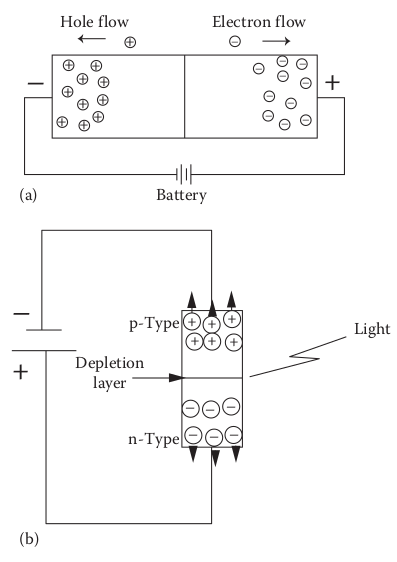
\includegraphics[width=0.55\textwidth]{2021-01-09_18-22.png}
    \caption{(a)反向偏置的p-n结,电池的正极连接n端;(b)光照射在耗尽区,光电
    二极管图例。}
    \label{fig:5.23}
\end{figure}

如果将二极管保持在反向偏压下,并且能量大于带隙能量的光子落在二极管结上(如图
\ref{fig:5.23}(b)所示),则会在耗尽区形成电子-空穴对。这些载流子将流过二极管,
产生的电流与落在二极管上的光的强度成比例。这些检测器涵盖从紫外线(约190 nm)到
近红外(约1000 nm)的光谱范围,但不如PMT灵敏。与PMT相比,它们的动态范围有限,
并且当它们偏离线性时,它们会急剧地变化。
\subsubsection{二极管阵列}
在UV/VIS光谱学中,可以通过扫描整个波长范围并用PMT记录光谱(一次是一个波长)来
获得完整的吸收光谱。尽管现代仪器比旧仪器要快得多,但是使用传统的扫描单色仪系统
需要花费时间。在与另一波长不同的时间测量一个波长的吸收。

在两种情况下,扫描光学系统不能很好地工作。首先是发生快速的化学反应,而常规扫描
太慢而无法追踪反应。第二个是样品仅在有限的时间内可用,而无法进行完整扫描。后者
的实例包括来自液相色谱分离的洗脱液,流动注射系统中的流动物流或化学或制药生产
厂中的工艺物流。在这种情况下,需要同时监视许多波长。理想情况下,应在同一时刻
测量整个光谱范围内的强度。如今,第三个条件常常推动了对快速分析的需求(在许多
行业中都要求高样品通量)通常是24/7全天候无人值守的仪器操作,这缩短了分析
“周转”时间并影响了成本。

线性PDA(LPDA)是开发用于能够同时测量许多波长的光强度的传感器。二极管阵列由嵌入
在一维线性阵列中的单晶中的许多半导体组成。常见的步骤是使用掺杂硅的单晶,它是
n型半导体。少量的IIIA族元素(例如砷)以规则的间隔嵌入到表面中。这产生了局部
p型半导体。半导体装置理想地具有如图\ref{fig:5.24}所示的横截面。该表面包含p–n结
的线性系列或阵列,每个结都是光电二极管。各个二极管称为元件,通道或像素。
\begin{figure}[htpb]
    \centering
    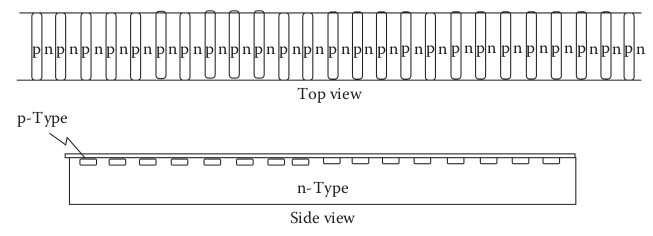
\includegraphics[width=0.85\textwidth]{2021-01-09_19-10.png}
    \caption{PDA}
    \label{fig:5.24}
\end{figure}

PDA布置为电路的一部分。通过给电路中的电容器充电,会在p-n结两端产生反向偏置。
辐射落在阵列上会在p和n区域产生电荷载流子。然后,电子将流向最近的p型半导体,并且
空穴被收集在p型区域中。电流使电容器部分放电。在测量周期结束时,电容器被充电;
充电电流产生的电压与光强度直接相关。在特定元件中形成的电荷载流子的数量取决于
该特定元件紧邻的阵列上的光强度。通过测量每个单独元素上的电荷,可以瞬时测量
光强度与整个光谱范围的波长的关系,但要测量离散的元素。这等于数字紫外线
吸收光谱。

商用多通道仪器的光学布局如图\ref{fig:5.25}所示。在此系统中,来自光源(可能是
氘灯或其他UV/VIS光源)的辐射穿过样品到达全息光栅,在全息光栅中,辐射被波长分开
并导向二极管阵列检测器。不使用出口狭缝。整个光谱区域的测量时间远远少于1 s。
实际上,光谱通常被采集超过1 s并由计算机存储。这种做法提高了测量的信噪比。通过
获取多个测量值,可以累积信号并显着提高灵敏度。
\begin{figure}[htpb]
    \centering
    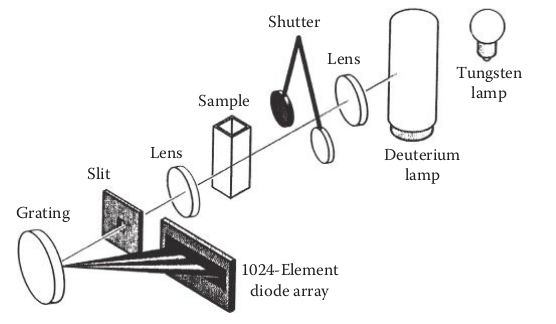
\includegraphics[width=0.85\textwidth]{2021-01-09_19-13.png}
    \caption{二极管阵列光谱仪光学系统}
    \label{fig:5.25}
\end{figure}

PDA可以覆盖190至1100 nm之间的波长范围。整个波长范围的同时使用提供了多路传输的
优势,并提高了系统的分辨率。系统的分辨率受所涉及的二极管元件数量的限制。典型的
二极管间距为0.025 mm。可以认为每个覆盖了有限的光谱范围。已经开发出了阵列中多达
4096个元素的检测器,尽管1024可能是最常见的数字。

二极管阵列系统最重要的应用是分子光谱,因为通常它们没有原子光谱所必需的分辨率。
在分子光谱学中,最有用的应用领域是(1)扫描快速反应以确定动力学;(2)涉及低光照
水平的应用,得益于光谱可以存储并相互添加,从而增加强度;(3)用于HPLC和毛细管
电泳(CE)的检测器。
\subsection{样品池}
用于UV/VIS光谱的样品可以是固体、液体或气体。针对这些样品类型设计不同类型的
样品池。如下一节所述,专为纳升样品量设计的新型光谱仪样品池。
\subsubsection{液相和气相池}
紫外线吸收或发射光谱学中使用的样品池或比色皿,必须对紫外线辐射透明。最常用的
材料是石英和熔融石英。石英和熔融石英对大多数溶剂也具有化学惰性,它们是坚固且
使用可靠。(注意:这些样品池中绝对不能使用含有氢氟酸或强碱的溶液,例如浓
\ce{NaOH}。此类溶液会腐蚀样品池表面,使其无法用于定量工作。)石英和熔融石英
样品池也是在可见光和NIR区域是透明的,因此这些可以用于UV和可见光区域的所有工作。
这些也是最昂贵的,因此,如果仅使用光谱的可见部分,则可以使用便宜的样品池,
例如Pyrex。

图\ref{fig:5.26}显示了一些典型的、多种尺寸的样品池类型。分光光度法的标准尺寸
一直是1 cm光程长的矩形样品池,该样品池可容纳约3.5 mL溶液,如图\ref{fig:5.26}
左上方所示。有体积小至40 $\mu$L的微体积池(图\ref{fig:5.26}左上角的第二个),
用于工艺流或大量样品常规分析的流通池,用于色谱系统的微流通池以及更大的气体和
高度稀释溶液的路径长度/容积池。图\ref{fig:5.26}底部中间显示了两个流通池。
通常,气室是长路径的气室,例如图\ref{fig:5.26}右上方所示的气室,一旦填充了气体
样本,气室必须能够关闭。样品池技术的创新包括纳米体积(即亚微升体积)的开发,
例如Starna可拆卸微体积(DMV)生物池,一种用于大多数UV/VIS光谱仪的超低体积池。
DMV-Bio的光程长度为0.5、0.2和0.125 mm,标称样品体积分别为2.5、1.0和0.6 $\mu$L。
另一个纳米体积的样品池是来自Hellma Analytics(www.hell-mausa.com)的TrayCell,
其路径长度为0.2或1.0 mm,可以测量和回收低至0.5 $\mu$L的体积(图\ref{fig:5.31}
)。
\begin{figure}[htpb]
    \centering
    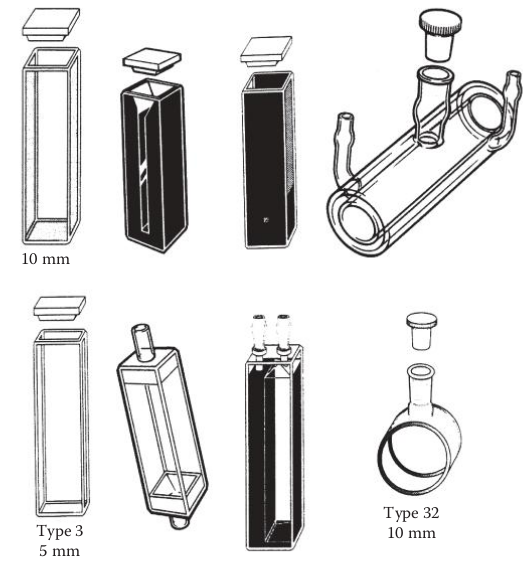
\includegraphics[width=0.75\textwidth]{2021-01-09_22-21.png}
    \caption{使用较广的液体样品池}
    \label{fig:5.26}
\end{figure}

为了在可见光谱范围内进行分光光度分析,可以使用玻璃或一次性塑料盒。它们比石英
或熔融石英便宜,但不能在短紫外线波长下使用。聚苯乙烯通常用于可见范围的比色皿
(340--800 nm),而丙烯酸聚合物比色皿可用于285 nm以下。塑料样品池不能与可溶于
塑料的任何有机溶剂一起使用。一次性塑料盒不适用于准确的定量工作。材料之间的价格
差异很大。例如,用于紫外线的高质量1 cm石英样品池的价格约为80美元,而透射范围为
220--3800 nm的1 cm Infrasil®石英样品池(来自Starna,Inc.)的价格约为130美元。
在可见区域使用的相同尺寸的玻璃样品池的价格约为35美元,而1 cm长的塑料一次性
样品池的价格约为10至20美分。微型样品池,流通池和其他专用细胞非常昂贵,每个
样品池的成本为200--500美元。一些光谱仪被设计为使用普通的玻璃试管作为“池”。
这些试管“池”不应用于准确的定量工作。图\ref{fig:5.27}显示了一些典型样品池材料
的透明度。
\begin{figure}[htpb]
    \centering
    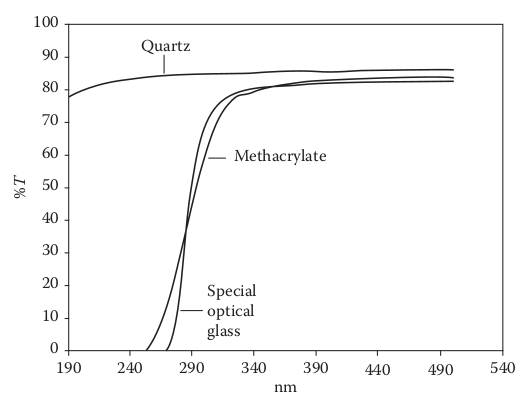
\includegraphics[width=0.75\textwidth]{2021-01-09_22-33.png}
    \caption{UV/VIS光谱样品池材质的透过率}
    \label{fig:5.27}
\end{figure}

重要的是正确处理样品池,以获得最佳结果并延长其寿命。为此,分析人员应(1)始终
选择正确的分析样品池;(2)保持样品池清洁并检查是否有污渍,蚀刻痕迹或划痕,这些
改变了电池的透明度;(3)将样品池应保持在不透明的表面上(如果提供);(4)使用前
彻底清洁,并在填充和测量之前用少量样品溶液润洗;(5)请勿将强碱性溶液或氢氟酸
(\ce{HF})溶液放入玻璃,石英或熔融石英电池中;(6)将一次性塑料样品池放入光谱仪
之前,检查其与溶剂的相容性;(7)对于非一次性电池,请务必小心干燥并返回其适当的
存储箱中;(8)切勿用纸制品,制造商推荐的镜头清洁纸或抹布擦拭光学表面。长期不
使用时,应保持样品池清洁干燥存放,以免刮伤光学表面。
\subsubsection{Matched Cells}
使用双光束仪器时,需要两个单元:一个用于参比,一个用于样品。这些样品池的吸收
略有差异是正常的。这会导致样品吸收率测量中的小误差,并可能导致分析误差。对于最
精确的定量工作,需要使用光学匹配的样品池。一个样品池的吸收等于或非常接近另一个
样品池的吸收。一次性准备大量样品池,并测量其各自的吸收率。具有非常相似的吸收率
的那些被指定为光学匹配的样品池。匹配的样品池通常在顶部附近刻有识别标记,必须
保持在一起。对于分析人员而言,重要的是要理解,由于原始材料特性的差异,即使是
匹配的样品池也会显示出很小的吸收差异。(由于正常使用,匹配样品池也会发生变化。
)可以使用不太常用的样品池(1 cm类型除外)以两个或四个单元的匹配集提供。匹配池
的正确使用是用溶剂填充样品池和参比池,并运行基线光谱,该光谱由仪器计算机系统
存储。然后清洗样品池并将样品溶液放入其中,同时将参比池及其溶剂留在原处。测量
样品光谱后,计算机会从样品光谱中减去基线。这种方法将纠正样品池的细微差异。同样
重要的是,将样品池以与获取背景时所面对的相同方向重新插入光谱仪。
样品池顶部的蚀刻标记有助于简化此过程。

现代样品池的制造已大大改善,像Starna这样的高品质样品池制造商现在正在生产比
旧的“匹配”样品池具有更好的窗平度、窗平行度、抛光度和光程长度精度的样品池。这些
现代样品池实际上可以通过制造过程的性质进行光学匹配,并且大量提供标准样品池(如
1 cm)。可在Starna网站(www.starna.com)上找到现代样品池的耐受性。分析人员仍然
有必要通过测量所有样品池中吸收材料的稀溶液来常规检查样品池。这将确定任何可能的
问题,包括细微的划痕,残留的薄膜或窗上的沉积物等。定性分析不需要匹配的样品池,
例如获得化合物的光谱以帮助鉴定其结构。
\subsubsection{直通采样器}
对于常规分析大量样品,大量样品池的填充、清洁和清空非常耗时。流通池和蠕动泵可用
于直接从其原始容器中测量样品溶液。提供样品量小至80 $\mu$L的流通池。消除了对
样品处理的需要,可以最大程度地减少样品处理带来的误差,并且不需要清洗许多样品池
。用于常规分析的流通式采样器在市场上有售。专用的进样系统和分段式进样系统可用于
特定常规分析,例如使用世界各地监管机构指定的方法(例如,《水和废水检验的标准
方法》中发现的方法)进行饮用水中的硝酸盐、硫酸盐和氟化物的分析。这些系统是自动
化的,可以采集样品,添加和混合试剂,并将吸收液通过固定波长的光谱仪进行完全无人
值守的定量分析。

多家仪器公司还提供stopped-flow附件,用于混合试剂和测量短期反应的动力学。安捷伦
科技公司提供的快速动力学配件,经验死区时间少于8 ms,与Cary分光光度计一起使用时
,可监测高达100 s$^{-1}$的反应速率,而使用的Cary分光光度计仅需350 $\mu$L试剂。
Thermo Fisher Scientific的Rapid Mix附件混合两种反应物,并使用低至120 $\mu$L的
反应物填充样品池,空载时间为8毫秒。流动回路和驱动注射器可以进行水温控,以进行
温度控制。样品表面具有化学惰性和生物相容性。通过改变注射器直径来改变反应物比率
。气动机构和软件触发功能可进行精确的零时间测量,并可测量从毫秒到分钟的反应
速率(图\ref{fig:5.29}(a))。
\subsubsection{固体样品架}
透明固体材料(例如聚合物)的薄膜的吸收光谱可通过使用薄膜固定器获得。最简单的
固定器类型可以是纸制载玻片架,样品粘贴在载玻片架上。然而,膜、凝胶和其他片材
的生产者通常对膜或片的均质性感兴趣。Cary系列光谱仪(Agilent Technologies, Inc.
)的胶片夹附件可安装长度最大为160 mm的样品。可以吸收光谱,然后自动移动样品,以
产生沿样品长度的吸收与位置的关系图。

凝胶电泳是分离高分子量(MW)生物分子,例如脱氧核糖核酸(DNA),脂蛋白,免疫球
蛋白和酶复合物。可视化分离分子的经典方法是用有色染料对其进行染色。可以将电泳
凝胶切片安装在固定器中(图\ref{fig:5.28}),并使用与移动膜样品相同的装置收集
沿凝胶距离的吸收光谱。支架可以以0.25 mm的增量移动,并且可以以这种方式分析长达
100 mm的凝胶。
\begin{figure}[htpb]
    \centering
    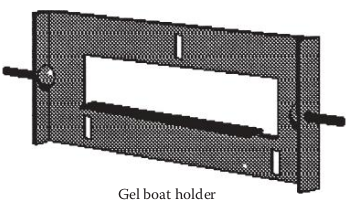
\includegraphics[width=0.45\textwidth]{2021-01-10_19-53.png}
    \caption{UV/VIS光谱用电泳凝胶样品架}
    \label{fig:5.28}
\end{figure}

有关傅里叶变换红外(FTIR)和近红外的描述,可以使用适当的附件通过漫反射或镜面
反射来测量固体样品。可以使用称为Praying Mantis(哈里克科学产品,
www.harricksci.com)的漫反射装置在光谱仪的整个波长范围内测量小至3 mm的固体和
粉末样品。它由两个大的半球形反射镜组成,可收集非常小的样品中的光,从而无需溶解
溶剂。对于材料科学和纳米材料,将1--2毫米厚,直径3毫米的粉末样品放在可吹扫室中,
因此可以研究对氧和水敏感的材料。可以在不同的条件下获得漫反射率测量值:温度
从$- 150^\circ$C到600 $^\circ$C,压力从10$^{-6}$ torr到3 atm。
\subsubsection{光纤探头}
在前面描述的所有样品池中,必须将样品放到光谱仪中并置于光路中(或泵入光路中)。
现代的光纤探头可以将光谱仪带到样品中。使用如图\ref{fig:5.29}(b)所示的光纤探针,
可以从微量离心管中很小的样品体积中收集吸收光谱。这些探头可覆盖200至1100 nm的
范围,并在高达150 $^\circ$C的温度下工作。光纤探头可用于从几乎任何容器内部收集
光谱,这些容器包括敞开的饮料罐,55加仑的材料桶,油罐车或充满液体的有轨电车。
探针的制作与样品池一样,具有各种路径长度,但无需收集样品并将其放入样品池中进行
测量。这对于未知和可能有害的样品尤其有用。光纤反射率和固定角度镜面反射率探头
可用于固体样品的远程测量。它们通常由316不锈钢制成,以易于清洁和相对惰性。
\begin{figure}[htpb]
    \centering
    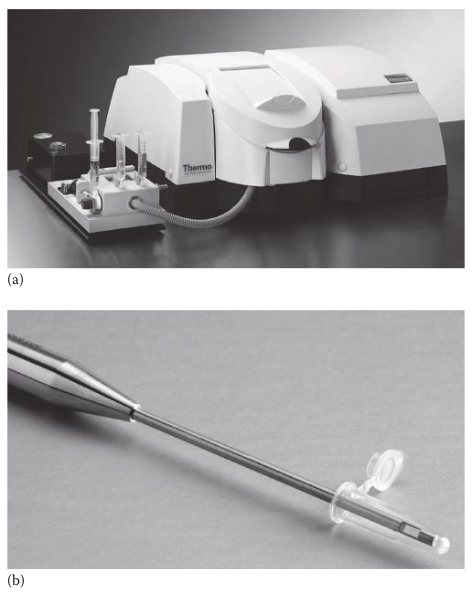
\includegraphics[width=0.65\textwidth]{2021-01-10_20-02.png}
    \caption{(a)用于快速动力学研究的UV/VIS光谱仪;(b)用于UV/VIS的光纤探头}
    \label{fig:5.29}
\end{figure}
\subsection{微量,纳米和手持式UV/VIS光谱仪}
近年来,人们对确定数量有限的生物样品中的DNA,核糖核酸(RNA),蛋白质等的浓厚
兴趣,以及化学实验室推动的减少样品和试剂量,从而减少浪费的强烈需求兴趣,在许多
实验室中,“对速度的需求”导致了各种微型体积UV/VIS仪器的开发,其中许多不需要样品
池,其中一些可以回收几乎所有样品。此外,与IR和Raman一样,手持设备现已出现,可以
在现场或制造厂进行分析。其中一些工具的示例,尽管这些工具并不全面,但已关注于
展示这些产品的各种创新。仪器本身将在本节中描述,而应用程序将在后续章节中讨论。

直接测量小体积样品的优点包括没有稀释误差,没有污染,没有样品制备时间或减少了
样品制备时间,并且增加了样品通量,尤其是在不需要样品池的情况下。随着光程长度的
减小,测得的吸光度会减小(Beer定律);因此,减小光程长度等同于样品稀释——
“虚拟稀释”。通过使用非常短的光程长度,无需稀释即可直接测量高吸收样品。如果需要
,这些仪器中的许多仪器都可以回收样品。

\subsubsection{微型系统}
NanoPhotometer\textsuperscript{TM}Pearl(来自Implen,GmbH; www.implen.com)
是一款紧凑型双通道Czerny Turner光栅光谱仪,带有1024像素电荷耦合检测器(CCD)
阵列检测器和氙气闪光灯光源(图\ref{fig:5.30})。
\begin{figure}[htpb]
    \centering
    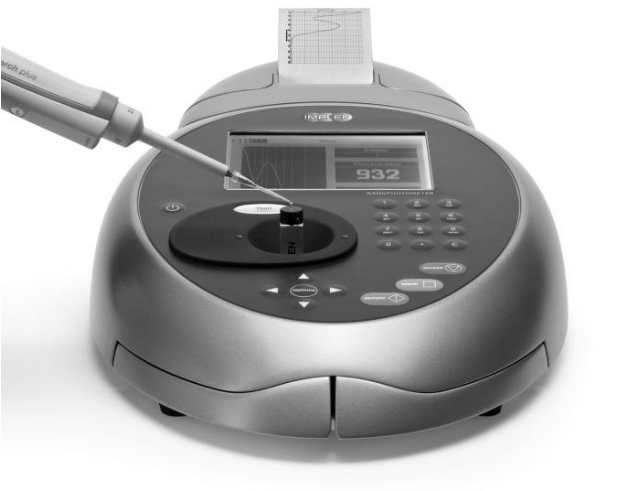
\includegraphics[width=0.75\textwidth]{2021-01-10_21-53.png}
    \caption{NanoPhotometer\textsuperscript{TM} Pearl}
    \label{fig:5.30}
\end{figure}

它的波长范围是190--1100 nm,能够在3.5 s内从200扫描到950 nm。该仪器不需要预热
时间,并且具有密封的光学元件和活动部件,因此无需重新校准。系统中最多可以存储
81种方法,并且系统附带了用于核酸(DNA,RNA)、蛋白质定量、细胞密度等方法的预定
义方法。该仪器既可以使用比色杯,也可以对比色杯小至0.3 $\mu$L的样品进行无比色杯
测量。这是通过Sample Compression Technology\textsuperscript{TM}
(www.implen.com/nanopho-tometer/how-it-works.php)完成的。将小至0.3 $\mu$L的
样品直接吸到光谱仪窗口中,并在滴液上方盖上盖子。盖子将样品挤压到精确定义的光程
长度,该路径长度与表面张力无关,并防止蒸发,如图\ref{fig:5.31}所示。
\begin{figure}[htpb]
    \centering
    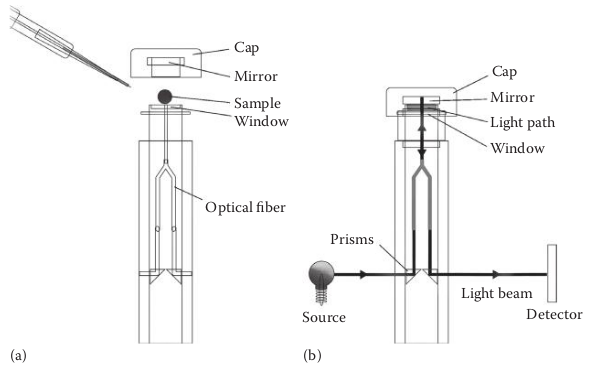
\includegraphics[width=0.85\textwidth]{2021-01-10_22-22.png}
    \caption{(a)将样品吸移至样品窗;(b)盖子将样品压至固定长度的光程中}
    \label{fig:5.31}
\end{figure}

提供五个不同的“虚拟稀释”盖,以提供精确的光程长度,分别对应于1/5、1/10、1/50、
1/100和1/250的稀释度。使用光纤,光源被引导向上穿过样品,并从帽中的反射镜反射
到检测器。测量后,可以用微量移液器取回样品,也可以将样品简单地从镜子和窗户上
擦掉。仪器选项卡下的应用程序,可在www.implen.de上查看仪器完整操作的视频。 
(注意:该样品池专利由Implen和Hellma Analytics共同拥有。只有Implen提供0.3 
$\mu$L选件和五个虚拟稀释盖。这些样品池的制造商Hellma Analytics提供了双重的虚拟
稀释版本TrayCell,即可直接从Hellma以及许多仪器公司获得,尽管通常使用
不同的名称。)
\begin{figure}[htpb]
    \centering
    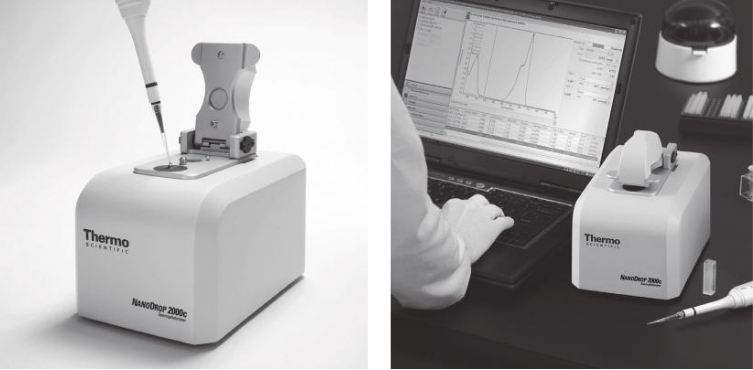
\includegraphics[width=0.95\textwidth]{2021-01-10_22-34.png}
    \caption{Thermo Scientific NanoDrop\textsuperscript{TM} 2000c}
    \label{fig:5.32}
\end{figure}

Thermo Fisher Scientific拥有一系列纳米体积光谱仪,即Thermo Fisher NanoDrop
\textsuperscript{TM}系列(图\ref{fig:5.32})。

NanoDrop\textsuperscript{TM}2000c是一款紧凑型(14$\times$20 cm)光谱仪,范围
为190--840 nm,测量时间$<$5 s,用于单一波长的吸光度,比色杯功能以及用于动力学
和细胞培养的加热和搅拌功能(图\ref{fig:5.32})。可以在整个光谱范围内测量
1--2 $\mu$L的样品。它也允许无比色杯测量,样品量低至0.5 $\mu$L。使用
NanoDrop\textsuperscript{TM},将样品直接移液到测量表面上,关闭盖子,并通过样品
在上下支座之间的表面张力(图\ref{fig:5.33}(a)和(b))形成“柱”。确切的体积并不
重要,只有形成一个色谱柱即可。移取样品,读取吸光度,并在15 s内将表面擦拭干净。
有关该操作的视频,请访问http://www.nanodrop.com/nd-1000-video.html和
nanodrop.com/HowItWorks.aspx。
\begin{figure}[htpb]
    \centering
    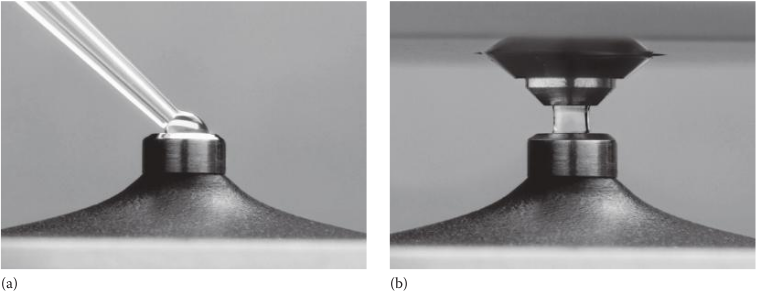
\includegraphics[width=0.95\textwidth]{2021-01-10_22-49.png}
    \caption{(a)将样品吸移至样品窗;(b)盖子将样品压至固定长度的光程中}
    \label{fig:5.33}
\end{figure}

使用96孔板的高通量实验室(图\ref{fig:5.34}(a)至(c))有8个样品版本。如图所示,
使用8通道移液器,可在约6分钟内运行96个样品。通过测量260和280 nm的吸光度,2012
年推出了掌上尺寸的新版本NanoDrop\textsuperscript{TM}Lite,用于专用核酸应用。 
大多数系统都具有用于生命科学的内置方法,包括核酸,蛋白质和比色蛋白质测定法,
例如Bradford和Lowry测定法。
\begin{figure}[htpb]
    \centering
    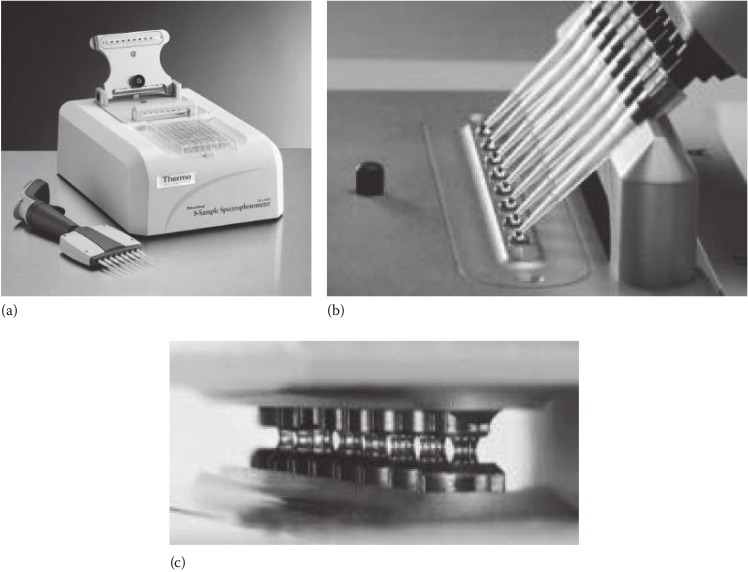
\includegraphics[width=0.95\textwidth]{2021-01-10_22-51.png}
    \caption{(a)将样品吸移至样品窗;(b)盖子将样品压至固定长度的光程中;(c)
    连续八组进样}
    \label{fig:5.34}
\end{figure}

AstraGene iCF UV/VIS分光光度计(AstraNet Systems, Ltd.,
www.astranetsys-tems.com; www.norsci.ca)是CCD阵列分光光度计,具有氙气光源,
并且光源和检测器通过光纤耦合。样品架,它是一个微型探针(图\ref{fig:5.35}(a)和
(b))。将2 $\mu$L样品吸在紫外线透明的一次性移液器吸头中。聚合物移液器吸头可透射
低至230 nm的紫外线,并具有固定的1 mm路径长度。通过移液器吸头进行吸光度测量
(图\ref{fig:5.35}(c)),将样品送回样品瓶,并丢弃吸头。这种“尖端技术”系统的
优点包括易于处理样品,没有样品残留或污染,无需清洁光学器件以及完全回收样品。
该系统旨在使用在260和280 nm处测得的吸光度对核酸和蛋白质进行常规分析,但是该
系统可以用作扫描UV/VIS分光光度计或以微阵列模式使用,在两个选定的位置测量吸光度
,浓度和两个选定波长的比率。核酸或蛋白质的测量大约需要2 s。
\begin{figure}[htpb]
    \centering
    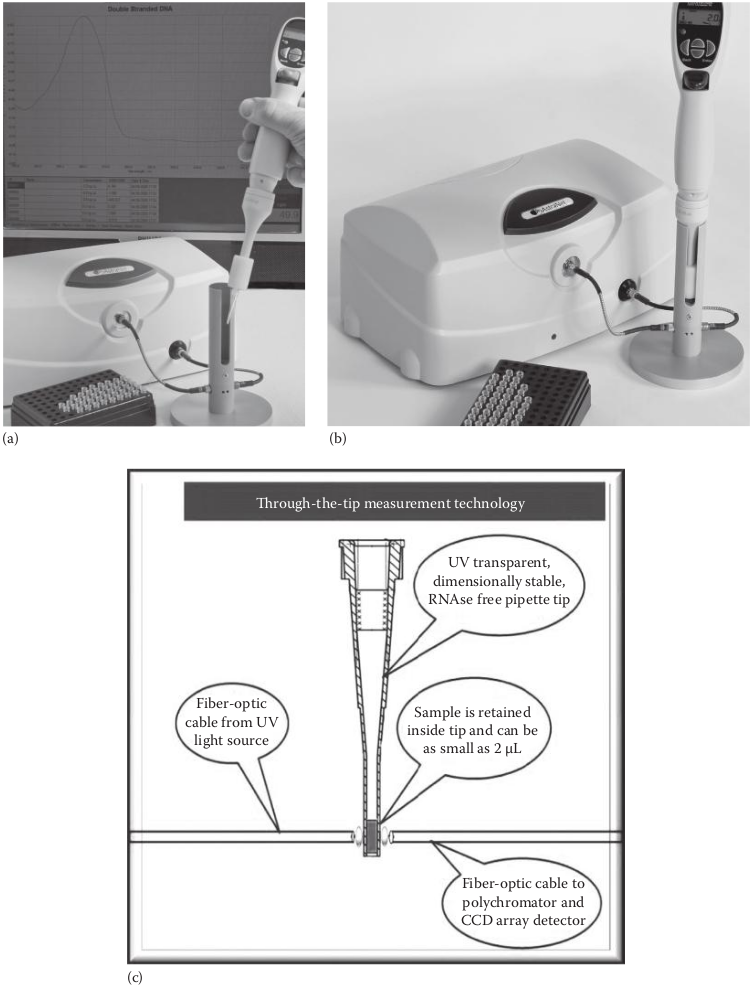
\includegraphics[width=0.95\textwidth]{2021-01-11_21-13.png}
    \caption{(a)AstraGene iCF UV/VIS光谱仪;(b)装有待测样的移液器;(c)
    “通过尖端”技术示意图}
    \label{fig:5.35}
\end{figure}
\subsubsection{可变光程斜率光谱仪系统}
吸收光谱通常使用固定的光程长度和标准品、样品的稀释液进行,以制备校准曲线并使
吸光度读数保持在线性范围内,如前一章所述。稀释液容易出错,可能会引起问题。从
高粘度浓溶液中稀释时,由于移液器通常不针对高粘度溶液进行校准。

C Technologies, Inc采用了一种新的UV/VIS/NIR光谱方法,将SoloVPE可变光程扩展,
并与Agilent Technologies, Inc的Cary 60分光光度计一起使用(图\ref{fig:5.36}(a)
)。 SoloVPE利用比尔定律中的路径长度术语,通过在0.005 mm(5 $\mu$m)--
15000 mm(1.5 cm)的范围内以5 $\mu$m的路径长度分辨率改变路径长度,从而允许在
同一样品中进行准确的测量。
\begin{figure}[htpb]
    \centering
    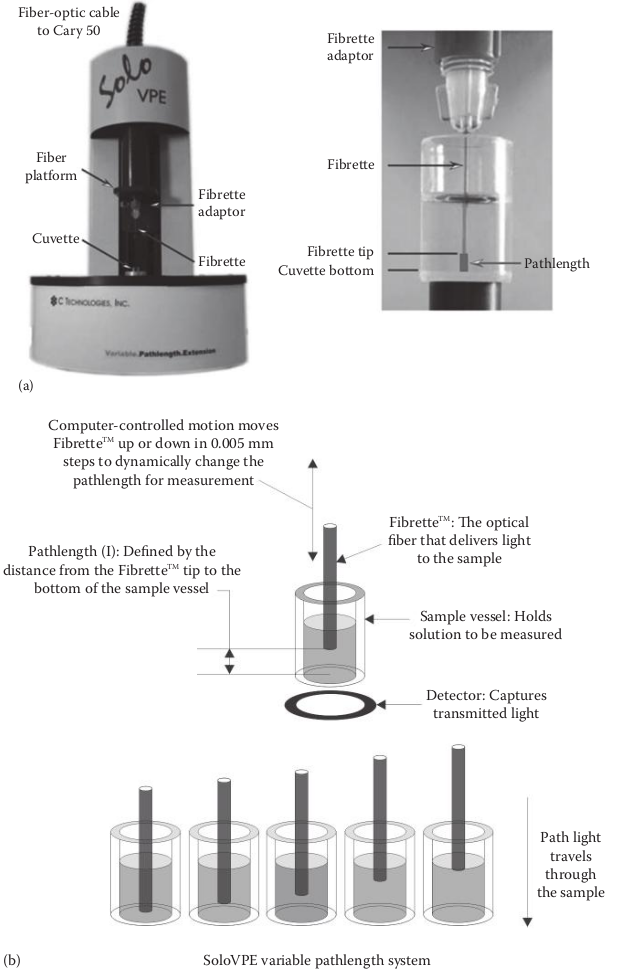
\includegraphics[width=0.85\textwidth]{2021-01-11_21-45.png}
    \caption{(a)左,SoloVPE,右,比色环和Fibrette\textsuperscript{TM};
    (b)SoloVPE工作原理,上是光纤通过样品池溶液将光传送到样品池底部的检测器,
    光程长度为Fibrette\textsuperscript{TM}尖端到样品池底部。
下是对Fibrette\textsuperscript{TM}位置的精确控制可提供多种光程;}
    \label{fig:5.36}
\end{figure}
\begin{figure}[t]
    \ContinuedFloat
    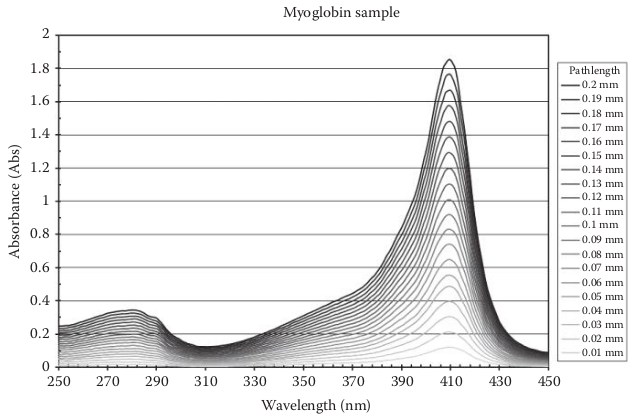
\includegraphics[width=0.85\textwidth]{2021-01-11_21-46.png}
    \caption{(c)20种不同光程长度测试肌红蛋白的吸收光谱,最长光程对应最高吸光度。}
\end{figure}

光纤电缆将光从分光光度计传输到SoloVPE中的光纤平台。光纤平台的末端是一次性的
单根光纤,称为Fibrette\textsuperscript{TM}。光线穿过Fibrette\textsuperscript{TM}
进入样品溶液(图\ref{fig:5.36}(b))。光纤可以相对于样品容器的底部上下移动,从而
改变可用的路径长度。控制路径长度的示例如图\ref{fig:5.36}(c)所示。在20个不同的
路径长度(从0.01到0.2 mm)中测量了一个肌红蛋白样品。随着光程长度的减小,吸光度
的降低表明仅通过移动Fibrette\textsuperscript{TM}即可对样品进行“虚拟稀释”。

Fibrette和容器由石英制成,波长范围为190-1100 nm;塑料容器也可用于UV或VIS–NIR
范围。可以测量最小的样品量(1-3 $\mu$L)并回收样品。

该技术的强大之处在于所绘制的情节。在任何给定的波长下,都可以绘制吸光度与路径
长度的关系图,称为波长截面图。与标准校准曲线一样,使用线性回归来提供回归方程。
波长截面图的回归方程m的斜率项,以Abs/mm为单位,在Beer定律的重排版本中使用,并
称为Slope Spectroscopy\textsuperscript{TM}方程:$m = A/l =\varepsilon c$,其中
$l$是光程长度。使用Slope Spectroscopy\textsuperscript{TM}公式,如果已知样品的
摩尔吸光系数,则可从$c = m /\varepsilon$获得浓度。同样,如果浓度是已知的,则
不仅可以在一个波长而且可以在许多波长下容易地获得摩尔吸收系数。来自此类图的斜率
可用于快速定量稀释比,并构建完整的消光光谱,同时使用不稀释的单个可回收样品。
1707 / 5000
Translation results
\subsubsection{手持式可见光谱系统}
Microspectral Analysis, LLC(www.microspectralanalysis.com)的i-LAB手持式可见
光谱仪是一款便携式微型光谱仪,由3个AA电池供电,覆盖400--700 nm区域,重量仅为
200 g(图\ref{fig:5.37})。该仪器的带宽为4--7 nm,光谱分辨率为1.4 nm,
没有活动部件。
\begin{figure}[htpb]
    \centering
    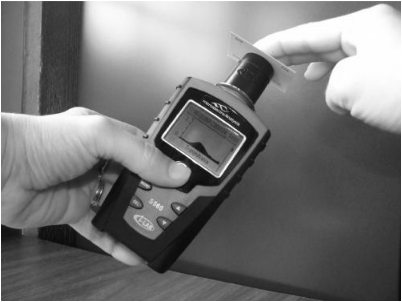
\includegraphics[width=0.75\textwidth]{2021-01-12_16-37.png}
    \caption{手持式光谱仪}
    \label{fig:5.37}
\end{figure}

i-LAB使用光谱平衡的LED来提供均匀的白光源,并带有线性耳式PDA检测器。光源穿过
液体样品并反射回来(图\ref{fig:5.38}),或直接从固体样品反射(图\ref{fig:5.37}
)并到达连接到多二极管阵列检测器的线性可变滤光片。在此传感器中,信号被波长
“合并”或分离,并从模拟信号转换为数字信号。光谱被记录并自动保存。使用Beer定律
计算,吸光度,透射率,曲线下面积,最大峰,峰比率,光谱匹配以及使用$l^\ast$、
$a^\ast$、$b^\ast$或Red-Green-Blue系统,将在应用程序中进行描述。一种新的系统
i-LAB$^\ast$LITE仪表不使用LED,而是使用阳光或人造光作为光源,并且可以用于温室
和商业光源的研究。
\begin{figure}[htpb]
    \centering
    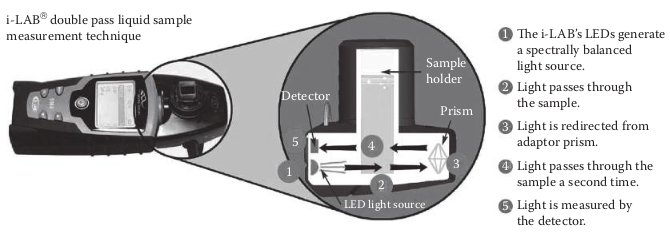
\includegraphics[width=0.95\textwidth]{2021-01-12_17-33.png}
    \caption{手持式光谱仪工作原理}
    \label{fig:5.38}
\end{figure}

该系统可提供多种样品适配器,包括比色皿架、圆形样品瓶架和用于液体的定制样品瓶,
以及用于固体的表面读取器。该软件允许用户创建定制的测量方法并将其传输到i-LAB。
应用将在后面章节中讨论。
\section{分子的紫外吸收光谱}
如前所讨论,UV/VIS吸收带的形状和强度,与吸收物质的电子构型有关。该讨论集中在
吸收与简单有机分子结构的关系。表\ref{tab:5.3}和\ref{tab:5.4}列出常用的有机
发色团、吸收UV/VIS的官能团的最大吸收峰。当然,发色团不是孤立的,它是分子的一
部分。通常分子溶解在有机溶剂中测量光谱。我们研究如何使用发色团的最大吸收峰和
一组准则来预测特定分子中的最大吸收峰的位置。我们还考虑溶剂如何影响某些分子的
光谱。有机分子吸收UV/VIS的跃迁是$n\to\sigma^\ast$、$\pi\to\pi^\ast$和
$n\to\pi^\ast$。
\subsection{一些术语}
这里需要定义一些术语。{\bf 发色团(chromophore)}是分子中吸收辐射的基团。{\bf 
助色团(auxochrome)}是分子中含有非键电子对(孤对电子)的基团,如\ce{OH}、\ce{NH}
和卤素。助色团可以使带有$\pi$电子的发色团的最大吸收峰的位置向长波长的方向移动。
这种向长波长方向移动,我们称之为{\bf 红移(red shift)};同理,向短波长方向移动,
我们称之为{\bf 蓝移(blue shift)}。吸收带强度增大(如$\varepsilon_{\text{max}}$
称为{\bf 增色(hyperchromism)},吸收强度减小称为{\bf 减色(hypochromism)}。波长
和强度的变化,是受整个分子结构,和溶剂与溶质的相互作用影响的。

最大摩尔吸光系数$\varepsilon_{\text{max}} \geq 10^4\text{ L}\cdot
\text{mol}^{-1}\cdot\text{cm}^{-1}$的吸收带称为{\bf 强带};
$\varepsilon_{\text{max}} < 10^3\text{ L}\cdot
\text{mol}^{-1}\cdot\text{cm}^{-1}$的吸收带称为{\bf 弱带}。

{\bf R带}是含有杂原子的发色团(如\chemfig{O=[,0.65]C(-[:10,0.5])(-[:-10,0.5])}、
\ce{-N=O}、\ce{-N=N-}等)
的$n\to\pi^\ast$跃迁所产生的吸收带。特点是强度较弱,一般情况下
$\varepsilon < 100\text{ L}\cdot\text{mol}^{-1}\cdot\text{cm}^{-1}$,吸收峰
通常位于200--400 nm之间。

{\bf K带}是由共轭体系$\pi\to\pi^\ast$跃迁产生的吸收带。其特点是吸收强度大,一般
$\varepsilon > 10^4\text{ L}\cdot\text{mol}^{-1}\cdot\text{cm}^{-1}$,吸收峰的
位置一般处于217--280 nm范围内。K带的吸收波长与共轭体系的数目、位置、取代基种类
等因素有关。共轭体系增加,红移,吸收强度也增加。可根据此特点,判断共轭体系存在
的情况。

{\bf B带}是芳香族化合物$\pi\to\pi^\ast$跃迁产生的精细结构吸收带。苯的B带摩尔
吸光系数约为$200 \text{ L}\cdot\text{mol}^{-1}\cdot\text{cm}^{-1}$,吸收峰在
230--270 nm之间,中心在259 nm,在极性溶剂中精细结构消失或不明显。

{\bf E带}同样是芳香族化合物$\pi\to\pi^\ast$跃迁所产生的吸收带,芳香族的特征吸收
,分为$E_1$和$E_2$带。如苯的$E_1$带出现在184 nm($\varepsilon=9000 \text{ L}
\cdot\text{mol}^{-1}\cdot\text{cm}^{-1}$),
$E_2$带出现在204 nm($\varepsilon=8000 \text{ L} \cdot\text{mol}^{-1}
\cdot\text{cm}^{-1}$)。
\subsection{溶剂的影响}
\subsubsection{红移}
相比于非极性溶剂,极性溶剂可使分子的$\pi\to\pi^\ast$跃迁发生红移。这不意味着
溶液变成红色,或者吸收发生在可见光谱的红色部分,仅是波长向光谱的红色或更长的
波长端移动。将样品溶于两种不同极性的溶剂中,可以用于确认分子中是否存在
$\pi\to\pi^\ast$跃迁。如果极性溶液中最大吸收峰的波长,比非极性溶液中的大,发生
红移。发生$\pi\to\pi^\ast$跃迁,分子中存在不饱和键。但,如果是二烯,或
其它多烯的$\pi\to\pi^\ast$跃迁,是不会受极性的影响而移动。

波长偏移与激发态能级有关。激发态的极性比基态的极性大,激发态与极性溶剂之间发生
相互作用,从而降低激发(吸收)能量。也就是说,在极性溶剂的作用下,基态与激发态
之间的能量差变小了,如图\ref{fig:5.39}所示。
\begin{figure}[htpb]
    \centering
    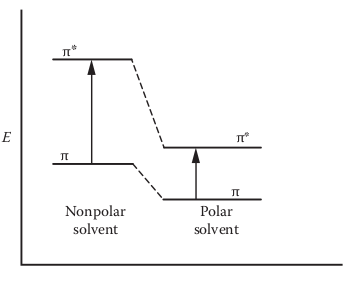
\includegraphics[width=0.55\textwidth]{2021-01-16_20-08.png}
    \caption{极性与非极性溶液中$\pi\to\pi^\ast$跃迁的不同能量}
    \label{fig:5.39}
\end{figure}

如果极性溶剂可以降低$\pi^\ast$的能量,那么,$n\to\pi^\ast$跃迁在极性溶剂中,也
会发生红移。但,事实不非如此。
\subsubsection{蓝移}
分子中存在\ce{O-H}和\ce{N-H}基团,分子间就会有氢键的作用。氢键比范德华力强,可
以说,是最强的分子间作用力。具有这样能力的溶剂,有水、醇(甲醇、乙醇)和包含
\ce{N-H}键的胺。

分子中,非键轨道的电子($n$电子)受氢键影响最大,导致$n$和$\pi^\ast$轨道之间
能量差变大。$n\to\pi^\ast$跃迁需要更大的能量,吸收峰发生蓝移,大约25--50 nm。
非键轨道能量降低的数值,几乎与氢键键能相当。溶剂的极性增加,甚至在非氢键(非
质子性)溶剂中,$n\to\pi^\ast$跃迁也会发生蓝移。这是由于非键电子溶解度增加,
溶剂化的电子能级降低。如果溶剂是非极性的,$n\to\pi^\ast$跃迁的能量要小于极性
溶剂或质子性溶剂中。

$\pi^\ast$能量的降低,对非键电子蓝移的影响远远大于红移。当含有非键(孤对)电子
的分子,溶解于乙醇中,发生$n\to\pi^\ast$跃迁吸收峰的位置,比溶解于正己烷的位置
,波长更短,发生蓝移。蓝移,只是表达吸收峰的位置向短波长方向移动,与是否吸收
蓝光无关。样品既可以溶解在非氢键溶剂(如正己烷)中,又可以溶解于氢键溶剂(如
乙醇)中。溶解于乙醇中的吸收峰,比溶解于正己烷的吸收峰的波长小,分子中存在非键
电子。$n\to\pi^\ast$和$n\to\sigma^\ast$跃迁,均可以通过氢键键和发生蓝移。200 nm
以上,几乎无法观察到$n\to\sigma^\ast$跃迁,若要观察到该蓝移,只能是真空的UV光谱
。

我们举一个蓝移的例子。一个同时包含$\pi$电子和非键$n$电子的分子,存在两个最大
吸收峰,当改变溶剂极性,可能同时发生红移和蓝移。通常,$\pi\to\pi^\ast$跃迁的
吸收强度是$n\to\pi^\ast$跃迁的10倍。这样的分子,溶解在正己烷这种非极性溶液中,
吸收光谱与图\ref{fig:5.40}相似。比较两个吸收峰的强度,假设250 nm处的吸收归属
为$\pi\to\pi^\ast$跃迁,350 nm处的吸收归属为$n\to\pi^\ast$跃迁,是由于前者的
吸光系数大于后者,前者的吸光度大约后者。
\begin{figure}[htpb]
    \centering
    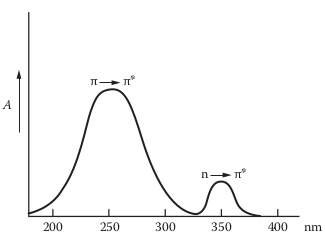
\includegraphics[width=0.65\textwidth]{2021-01-19_22-59.png}
    \caption{非极性溶剂中$\pi\to\pi^\ast$和$n\to\pi^\ast$跃迁}
    \label{fig:5.40}
\end{figure}

如果溶解在乙醇这种极性、氢键键和溶剂中。溶剂的极性会使$\pi\to\pi^\ast$跃迁发生
红移,而氢键键和会使$n\to\pi^\ast$跃迁发生蓝移,如图\ref{fig:5.41}所示。
\begin{figure}[htpb]
    \centering
    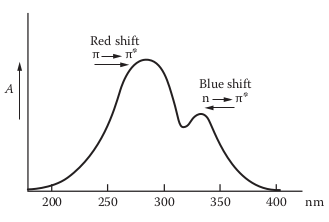
\includegraphics[width=0.65\textwidth]{2021-01-19_23-02.png}
    \caption{极性溶剂中$\pi\to\pi^\ast$跃迁(红移)和$n\to\pi^\ast$跃迁(蓝移)}
    \label{fig:5.41}
\end{figure}
\section{有机分子的紫外光谱和结构}
多年来,在实验数据基础上建立经验法则,将UV吸收最大值的波长与分子的结构相关联。
R. B. Woodward在1941年,L. Fieser和M. Fieser制定了规则,通过研究萜烯,类固醇
和其他天然产物来预测二烯,多烯和共轭酮的最大吸收量。该规则称为伍德沃德规则
(Woodward's rule)或伍德沃德·费塞尔规则(Woodward-Fieser rules)。

基本上有四个感兴趣的有机分子系统,主要的母体染色体系统是(1)共轭二烯;(2)单取代
的苯环;(3)二取代的苯-烯环和(4)共轭的羰基系统。计算方法是识别母系统并分配最大
吸收。然后通过分子中其他系统的存在来修饰母体系统。通过这些修改,可以计算出特定
分子结构的最大吸收。
\subsection{共轭二烯体系}
共轭二烯主体结构为\ce{C=C-C=C},在正己烷溶剂中的最大吸收峰为217 nm。每增加一个
共轭,最大吸收波长增大30 nm。相似的,每增加一个烷基,共轭体系最大吸收波长增大
5 nm。其它基团,如烷氧基、环内和环外双键,都可以增大最大吸收峰位置。表
\ref{tab:5.6}列出这种影响,需要强调的是,这只是实验数据总结的经验,而非理论。
\begin{table}[htbp]
    \centering
    \caption{吸收峰计算的经验法则}
    \label{tab:5.6}
    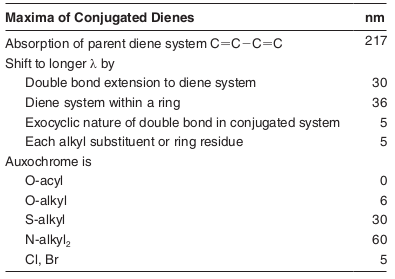
\includegraphics[width=0.6\textwidth]{2021-01-20_14-40.png}
\end{table}

\begin{example}
    \begin{figure}[htpb]
        \centering
        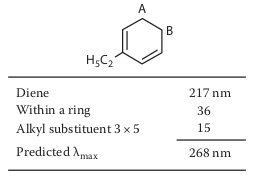
\includegraphics[width=0.5\textwidth]{2021-01-20_18-17.png}
        \label{fig:ex5.1}
    \end{figure}
具有二烯结构的六元环,二烯的碳原子上有一个烷基。预测该结构最大吸收峰为268 nm。
参照表\ref{tab:5.6}数据,二烯主体结构为217 nm,二烯结构在环上,加上36 nm。
三个烷基不容易很理解,其中一个乙基很清晰,A和B两个位置也是两个烷基。A、B两个
碳原子从两侧附着在二烯的两侧,分散电子密度,导致红移。每个烷基影响加5 nm,所以
,最大吸收峰将出现在$217 + 36 + 3\times 5 = 268$ nm。
\end{example}
\begin{example}
    \begin{figure}[htpb]
        \centering
        \includegraphics[width=0.4\textwidth]{2021-01-20_18-40.png}
        \label{fig:ex5.2}
    \end{figure}
比上一个例子稍微复杂一点。主体二烯依旧是217 nm。二烯也在环上,加36 nm。有一个
双键扩展了共轭体系,一共三个双键,加30 nm。C和D两个碳原子之间的双键,归属为
环外双键,加5 nm。这个双键在两个环的相邻处,属于共轭体系。E和F两个碳原子之间的
双键也在环内,但两个碳原子都不与另外环相邻,所以这个双键不属于环外双键。A和B
之间的双键与此相同。有五个烷基,碳原子A上有两个、碳原子B上有一个、碳原子D上有
一个和碳原子F上的一个。最大吸收峰将出现在$217+36+30+5+25=313$ nm。
\end{example}
\begin{example}
    \begin{figure}[htpb]
        \centering
        \includegraphics[width=0.4\textwidth]{2021-01-20_20-18.png}
        \includegraphics[width=0.4\textwidth]{2021-01-20_20-18_1.png}
        \label{fig:ex5.3}
    \end{figure}
两个分子相似,但结构不同,主要是双键位置不同。左侧最大吸收峰比右侧大66 nm,主要
是因为左侧结构同一环中的两个双键与第三个双键形成共轭。环内二烯,加36 nm,环外
共轭双键,加30 nm。右侧结构,尽管也有三个双键,但没有共轭结构。右上的双键与
二烯的双键间隔两个单键。右侧分子中,对最大吸收有贡献的结构是环外双键和烷基。
\end{example}
\begin{example}
    \begin{figure}[htpb]
        \centering
        \includegraphics[width=0.45\textwidth]{2021-01-20_23-24.png}
        \label{fig:ex5.3}
    \end{figure}
此结构最大吸收峰在235 nm。没有同环二烯结构,单环中没有完整的二烯。碳原子B的双键
不是环外双键。
\end{example}
\subsection{共轭酮}
共轭酮的主体结构为
\begin{figure}[h!]
    \centering
    \includegraphics[width=0.2\textwidth]{2021-01-22_15-20.png}
\end{figure}

最大吸收波长在215 nm。与共轭二烯规则相似,通过扩展双键取代、相对于环和相对于
羰基的位置,来改变共轭酮最大吸收峰的波长。碳原子分别标记为$\alpha$
、$\beta$、$\gamma$和$\delta$,这些位置的取代改变最大吸收峰的位移。如表
\ref{tab:5.7}是用于计算不同化合物最大吸收峰的经验值。
\begin{table}[htbp]
    \centering
    \caption{$\alpha$,$\beta$-不饱和醛酮吸收规则}
    \label{tab:5.7}
    \includegraphics[width=0.7\textwidth]{2021-01-22_15-45.png}
\end{table}
\begin{example}\label{ex:5.6}
    \begin{figure}[h!]
        \centering
        \includegraphics[width=0.35\textwidth]{2021-01-22_15-48.png}
        \caption{例\ref{ex:5.6}结构图}
    \end{figure}
只有附着在母体结构上的取代基才能对最大吸收产生影响。此例中$\delta$碳原子有两个
烷基取代,加36 nm,$\gamma$碳原子有一个取代基,加18 nm。$\gamma$和$\delta$之间
双键不是环外双键,它在两个环内,不属于任何环的环外双键。羟基不与主体结构相连,
不影响吸收。
\end{example}
\begin{example}\label{ex:5.7}
    \begin{figure}[h!]
        \centering
        \includegraphics[width=0.35\textwidth]{2021-01-22_15-50.png}
        \caption{例\ref{ex:5.7}结构图}
    \end{figure}
此例与上例互为异构体。所计算的最大吸收峰为286 nm。多种位置与上例有异。如,
$\delta$位只有一个烷基取代基;$\gamma$和$\delta$之间的双键是环外双键,可使吸收
红移。共轭体系不在环内。
\end{example}
\begin{example}\label{ex:5.8}
    \begin{figure}[h!]
        \centering
        \includegraphics[width=0.35\textwidth]{2021-01-22_15-51.png}
        \caption{例\ref{ex:5.8}结构图}
    \end{figure}
此例计算结果与上例相同,都是286 nm。计算步骤与上例相同。需要强调的是,与共轭
结构或母体结构不相连的分子部分,不影响吸收。
\end{example}

基于结构预测最大吸收峰的想法,是希望吸收光谱能够告诉我们未知物质的结构。但从
例\ref{ex:5.7}和\ref{ex:5.8}两个例子证明,不可能利用紫外光谱的最大吸收峰来
判断分子结构。
\subsection{苯环上的取代基}
苯是紫外的强吸收剂,尤其在气相中,苯显示出相当大的精细结构,如图\ref{fig:5.11}
。苯环上的取代基导致吸收峰的位移。经常可以观察到苯的紫外吸收的两个谱带,表
\ref{tab:5.8}和\ref{tab:5.9}给出一些取代苯环的最大吸收峰。这些只是实验数据,不
足以完全鉴定未知化合物。如果苯环上发生二取代,则必须进行计算,才能预测最大
吸收峰的位置。如下一些规则帮助我们理解苯的二取代:
\begin{enumerate}
    \item 邻位或对位的电子接受体,如硝基,和电子给予体,如羟基,往往会相互抵消
        ,并且提供的光谱与单取代苯环光谱没有很大的不同,见表\ref{tab:5.8};
    \item 两个彼此对位的电子接受体或两个电子给予体,所得的光谱与单取代几乎相同
        ;
    \item 彼此对位的电子接受体和电子给予体引起红移,见表\ref{tab:5.9}中苯的
        对二取代。
\end{enumerate}
\begin{table}[htbp]
    \centering
    \caption{苯环单取代的最大吸收峰}
    \label{tab:5.8}
    \includegraphics[width=0.75\textwidth]{2021-01-22_17-12.png}
\end{table}
\begin{table}[htbp]
    \centering
    \caption{苯环二取代的最大吸收峰}
    \label{tab:5.9}
    \includegraphics[width=0.75\textwidth]{2021-01-22_17-13.png}
\end{table}
\begin{example}
\begin{tabular}{c}
\includegraphics[width=0.5\textwidth]{2021-01-22_17-15.png}
\end{tabular}
\end{example}
\section{分析的应用}
\subsection{定性结构分析}
可以发生UV吸收的结构为非键($n$)电子和共轭双键($\pi$),如芳香化合物和共轭烯烃。
这些结构的吸收,集中在同一个较小的波长范围内,吸收光谱有重叠。定性分析的第一步
是样品的提纯,消除杂质的吸收带。即使是纯化后的样品,光谱也经常是宽峰,没有精细
结构。由此,在定性分析中,紫外吸收并不能像MS、IR和NMR那样有用。如今,实验室中,
很少用紫外吸收光谱来确定有机物的结构。

紫外吸收用来定性,通常是采取对比已知和未知化合物的吸收光谱的方法。定性UV/VIS
光谱在快速筛选样品领域依然非常有用。在高通量的环境中,可以定性地使用UV吸收来
筛选可能含有高含量的有机化合物样品,以避免污染敏感仪器。

另一种定性方法是使用导数光谱,即绘制吸光度光谱的一阶、二阶甚至更高的导数。导数
光谱可以增强光谱之间的差异,分解重叠的谱带,并减少来自其他吸收化合物的干扰的
影响。带的数量随着导数的高阶而增加。导数谱的复杂性增加可能有助于化合物鉴定。
例如,睾丸激素的吸收光谱显示一个单一的宽峰,中心在330 nm附近。二阶导数光谱具有
六个不同的峰。
\subsection{定量分析}
紫外和可见吸收光谱法是进行定量分析的有力工具。它用于化学研究、生物化学、化学
分析和工业加工。定量分析基于吸收程度和吸收材料浓度之间的关系。在数学上,我们
已经讨论Beer定律$A = \varepsilon lc$对许多化学系统的描述。通过测量强度比应用于
定量吸收光谱法的术语是分光光度法。在光谱的可见区域中使用分光光度法通常被称为
比色法。为避免混淆,当需要定量确定分析物种类时,术语“分光光度法”应同时用于紫外
和可见光区域。定性分析对于有机分子以及某些过渡和稀土化合物最有用,而定量UV/VIS
分光光度法则可用于确定有机分子、无机分子、金属和非金属离子以及有机金属络合物。

UV/VIS分光光度法是一种广泛使用的分光技术。它已在世界各地广泛用于研究,临床分析
、工业分析、环境分析和许多其他应用。紫外线吸收光谱的一些典型应用包括环境测试中
饮用水中苯酚,非离子表面活性剂,硫酸盐,硫化物,磷酸盐,氟化物,硝酸盐,多种
金属离子和其他化学物质,类固醇等天然产物的浓度测定或生物化学中的叶绿素,染料
材料以及维生素,蛋白质,DNA和酶。

定量UV/VIS分光光度法已用于测定有机样品中的杂质,例如使用流通池的工业工厂物流中
的杂质。例如,它可用于测定痕量的简单烯烃中的共轭烯烃或纯己烷或类似链烷烃中的
芳族杂质。它也已用于检测食品,饮料,香烟烟雾和空气中可能的致癌物质。在农业领域
,UV/VIS分光光度法用于测定含氮和磷的肥料。在医学领域,它用于测定酶,维生素,
激素,类固醇,生物碱和巴比妥酸盐。这些测量值可用于诊断糖尿病,肾脏损害和心肌
梗塞以及其他疾病。在制药工业中,它可用于测量制造过程中药物的纯度和最终产品的
纯度。例如,阿司匹林,布洛芬和咖啡因是止痛片中的常见成分,它们都在紫外线下吸收
,可以通过分光光度法轻松测定。

例如,对乙酰氨基酚\ce{C8H9NO2}的纯度可以通过测量药物水溶液在244 nm处的吸光度
并将其与已知纯度和浓度的对乙酰氨基酚溶液进行比较来确定。有关详细信息,请参见
本章末尾建议的实验。

通常通过UV/VIS分光光度法对食品和饮料进行分析,以确保质量并确定杂质。这种分析的
一个例子是蜂蜜中羟甲基-糠醛的含量测定。该方法在Keppy等人的参考文献中进行了描述
。HMF是在酸性条件下果糖分解产生的醛。它的发色团在284 nm处吸收。尽管大多数蜂蜜中
的HMF随时间自然发生,但高含量的HMF可能表明储存条件差,掺糖添加剂或高热量。

橄榄油是许多国家的主要农产品。它比其他蔬菜油更有价值,尤其是高等级的特级初榨
橄榄油(EVOO),但在过去的20年中,世界各地有很多案例发现EVOO会掺入廉价的油,例如
葵花籽油、低芥酸菜籽油和大豆油(Claverie和Johnson,及其中的参考文献)。评估
橄榄油的标准方法是使用酚酞滴定酸度。这是一种缓慢的方法,可以将掺假样品的
结果“合格”。显然需要对EVOO进行快速,准确的测试。由于存在于橄榄中的色素(主要是
叶绿素和类胡萝卜素),橄榄油具有多种绿金色。Claverie和Johnson使用手持式i-LAB
可见光谱仪,使用5 cm比色杯在400--700 nm范围内测量了12种食用油。发现EVOO样品在
417、455、478和667 nm处具有主要吸收峰(图\ref{fig:5.42}),而低芥酸菜子油和
混合油则没有这样的吸收峰。图\ref{fig:5.42}中在400 nm处吸光度小于0.45的四个光谱
中的三个是已知的非EVOO样品。但是,这四个光谱中显然没有包含特征吸收峰的光谱
之一来自标有EVOO的样品。可见光谱可以在大约10 s内清晰,快速地识别出橄榄油。此外
,i-LAB在获取光谱的同时提供了CIE三刺激色值,如下所述。

紫外分光光度法测定核酸和蛋白质是一项主要应用,正如我们已经看到的那样,系统现在
能够对0.3--2 $\mu$L的样品量进行这种测定,通常是非破坏性的。这对于DNA微阵列,
PCR和法医DNA测量至关重要。核苷酸中的含氮碱基,嘌呤和嘧啶在260 nm的$\lambda_
{\text{max}}$处吸收。使用已知的消光系数,可以确定双链DNA(dsDNA),单链DNA和
RNA的浓度。使用前面描述的微体积系统,可以在大约2--18000 ng/$\mu$L的范围内测量
dsDNA。由于芳香族氨基酸色氨酸,酪氨酸,苯丙氨酸以及较小程度的二硫键,蛋白质和
多肽在280 nm处强烈吸收。DNA样品在280 nm处的吸光度估计了样品中蛋白质的浓度,
260 nm处的吸光度与280 nm处的吸光度之比是DNA样品纯度的量度。该比率应在1.65和
1.85之间。考虑到蛋白质和多肽作为疾病的治疗剂的使用越来越多,在280 nm处蛋白质和
多肽的测量本身就是重要的应用。消光系数测定法是在线性工作范围内确定消光系数的
方法,可用于鉴定蛋白质和肽。基于溶液中染料和蛋白质之间复合物的形成,还有许多
经典的分光光度法蛋白质分析方法。参考书目中引用了命名的测定法。 Bradford分析
基于考马斯亮蓝(Coomassie Brilliant Blue)G-250从465 nm到595 nm的位移。这种转变是
由于染料与蛋白质结合后阴离子形式的稳定化。二辛可宁酸(BCA)分析(Smith等人)是
基于蛋白质和碱性铜离子与BCA的反应,形成紫色复合物,其最大吸收在562 nm处。
\begin{figure}[htpb]
    \centering
    \includegraphics[width=0.85\textwidth]{2021-01-22_19-59.png}
    \caption{多种蔬菜油的吸收光谱}
    \label{fig:5.42}
\end{figure}

许多临床化学分析都是基于UV/VIS分光光度法的,通常是通过使感兴趣的化学物质(例如
葡萄糖)与酶和染料发生反应来生成有色复合物。中佛罗里达大学国家司法科学中心的
研究人员使用Implen NanoPhotometer\textsuperscript{TM}Pearl(Hanson和Ballantyne)
开发了一种确定犯罪现场干燥血迹年龄的新方法。研究人员在血红蛋白的Soret带(
$\lambda_{\text{max}}$= 412 nm)中发现了一个以前无法确定的蓝移,与干血迹沉积的
时间具有高度相关性。这种变化的程度使得可以区分在恢复和分析之前几分钟,几小时,
几天和几周沉积的血迹。可以在小至1 $\mu$L的血迹上进行测试,并且可以通过在
NanoPhotometer上收集血红蛋白UV/VIS光谱来确认斑点为血液。

尽管许多经典的分光光度测量方法已被诸如离子色谱法(IC),原子光谱法之类的仪器方法
所取代,但通常还是使用分光光度法来测定各种样品中金属和非金属离子的浓度。光谱
紫外区中的分光光度法可用于直接测量许多有机化合物,尤其是具有芳香环和共轭多键
的有机化合物。也有无色的无机物质吸收紫外线。硝酸根离子\ce{NO^3-}是一个很好的
例子。通过测量220和275 nm处水的吸光度,可以快速筛查饮用水中的硝酸盐。硝酸根离子
在220 nm处吸收,但在275 nm处不吸收;275 nm处的测量是为了检查可能存在的干扰
有机化合物。每当样品着色时,都可以使用可见光区域的分光光度分析。许多材料固有地
着色而没有化学反应(例如,无机离子,例如重铬酸根,高锰酸根,铜离子和铁离子),
并且不需要进一步的化学反应即可形成有色化合物。有色有机化合物(例如染料)也可以
自然着色。这种材料的溶液可以直接分析。然而,大多数金属和非金属离子是无色的。
这些离子在样品溶液中的存在可以通过首先使离子与有机试剂反应形成强吸收性物质来
确定。如果反应产物是有色的,则可以在可见光区域测量吸光度。或者,形成的产物可以
是无色的,但在紫外线中吸收。随着分析物浓度的增加,大多数分光光度法测定结果会
导致吸光度增加(如果可见,颜色会更暗)。但是,有些分析会随着分析物浓度的增加而导
致颜色褪色(吸光度降低)。

如引言中所述,我们在有色溶液中观察到的颜色是溶液透射的颜色。被吸收的颜色是
互补色。表\ref{tab:5.10}给出了吸收的光的颜色与观察到的颜色之间的关系。
\begin{table}[htbp]
    \centering
    \caption{吸收和观察的颜色}
    \label{tab:5.10}
    \includegraphics[width=0.45\textwidth]{2021-01-22_21-38.png}
\end{table}

通过使分析物种类与有机试剂反应可以形成数千种可能的化合物和络合物。理想情况下,
选择的试剂应具有选择性;也就是说,在当前条件下,它只能与一个离子或分子发生反应。
其次,与分析物混合时,试剂应引起突然的颜色变化或吸光度变化。这赋予该方法高灵敏
度。第三,这种颜色强度或紫外线吸收强度应与样品中离子的浓度有关。已经开发了用于
几乎所有金属和非金属离子以及用于许多分子或分子类别(即用于官能团)的分光光度
试剂。这些反应中许多都是敏感的和选择性的。这些试剂及其用途的几个例子在表
\ref{tab:5.11}中给出。参考书目中列出的Boltz以及Sandell和Onishi的书是经典参考
书目,但可能很难找到。分析文献包含数千种直接和间接的金属和非金属定量分析方法。
参考书目中列出的Dean的手册中提供了有关大多数金属和非金属离子的文献参考方法的
良好摘要。
\begin{table}[htbp]
    \centering
    \caption{用于光谱的典型试剂}
    \label{tab:5.11}
    \includegraphics[width=0.95\textwidth]{2021-01-22_21-58.png}
    \includegraphics[width=0.95\textwidth]{2021-01-22_22-00.png}
\end{table}

通过吸收分光光度法进行的定量分析要求样品中没有颗粒,即没有浊度。其原因是粒子会
散射光。如果样品散射的光远离检测器,则被解释为吸光度。如果样品浑浊,吸光度会
错误地高。如后续章节所述,我们可以利用光的散射来表征样品,但是必须避免使用颗粒
以进行准确的吸光度测量。

通过分光光度法进行定量分析通常需要针对所有标准品,样品和空白样品使用相同的pH
条件,添加的试剂等来准备校准曲线。包含所有已添加到样品中的所有试剂(分析物除外
)的空白试剂至关重要。测量所有空白,标准品和样品的吸光度。从所有其他吸光度中
减去空白的吸光度,并从标准品构建校正曲线。根据校准曲线确定样品中分析物的浓度。
在校准曲线的线性区域内工作可获得最高的精度。这些定量方法在所涉及的化学过程中
非常复杂,并且需要进行许多步骤(方法中可能涉及萃取,反萃取,pH调节,沉淀,
掩蔽和许多其他类型的操作),并且分析人员必须注意所有细节,以达到准确和精确的
结果。许多分析都涉及科学和艺术。
\subsection{多组分检测}
UV/VIS吸收峰是宽峰,如果溶液中有两种化合物X和Y,两种物质在相同的波长,都有吸收
,将无法分辨出来。可以通过一系列测量来计算X和Y的浓度(必须在等于混合物中组分
数量的多个波长下进行测量)。在这种情况下,有两个分量,需要两个波长。两个组分
都要遵循Beer定律,并且两个组分在溶液中不发生相互作用,他们的吸光度是累加的。

需要准备四条标准曲线:X在$\lambda_1$、X在$\lambda_2$、Y在$\lambda_1$和Y在
$\lambda_2$。所有曲线均应做空白校正,并通过原点。在$\lambda_1$和$\lambda_2$
下测量样品混合物的吸光度,等式可写做:
\begin{equation}
    \begin{array}{rcl}
    A_1 &=& C_X S_{X1} + C_YS_{Y1}\\
    A_2 &=& C_X S_{X2} + C_YS_{Y2}
\end{array}
\label{5.3}
\end{equation}
$A_1$未知物在$\lambda_1$处的吸光度;$A_2$未知物在$\lambda_2$处的吸光度;
$C_X$未知物中X的浓度;$C_Y$未知物中Y的浓度;$S_{X1}$是X在$\lambda_1$处吸收的
标准曲线的斜率;$S_{X2}$是X在$\lambda_2$处吸收的标准曲线的斜率;
$S_{Y1}$是Y在$\lambda_1$处吸收的标准曲线的斜率;$S_{Y2}$是Y在$\lambda_2$处吸收
的标准曲线的斜率。

吸光度和斜率是已知的,两个等式,两个未知数$C_X$和$C_Y$,可解出浓度。
Dulski提供这种方法的示例,该方法通过与对苯二酚反应并在400和500 nm处同时测定
铌和钛。另一个例子是分析含有1-苯肾上腺素(PEH)和马来酸氯苯那敏(PAM)的常见鼻
喷雾剂。水溶液中的每种化合物在紫外线下均具有较宽的吸收峰。选择两个波长:如果
可能,最好选择每个波长的$\lambda_{\text{max}}$。鼻喷雾剂中两种成分的量可以通过
准备每种化合物的校准曲线,获得线在两个波长(例如在266和272 nm)处的斜率来找到。
如前所示,这给出了四个S项。然后,在两个波长下测量样品,得出A项。本章末尾的建议
实验中概述了该实验。

相同的方法可以用于三种成分的混合。可以通过计算机软件解散更复杂的混合物,该软件
使用多个波长的迭代过程来计算浓度。所使用的数学方法包括偏最小二乘(PLS),多重最
小二乘,主成分回归和其他统计方法。使用紫外线吸收的多组分分析已被用于确定蛋白质
中存在多少种芳香族氨基酸,以及哪种类型的芳香族氨基酸用于定量
血液中五种不同的血红蛋白。
\subsection{其它应用}
\subsubsection{反应动力学}
与其他光谱技术一样,紫外光谱可用于测量化学反应的动力学,包括酶催化的生物化学
反应。例如,假设两种化合物A和B反应形成第三种化合物C。如果第三种化合物吸收
紫外线,则可以连续测量其浓度。可以在实验开始时测量A和B的原始浓度。通过在不同
时间间隔测量C的浓度,可以计算出反应$A + B\to C$的动力学。酶的反应在生化和分析
上都很重要。对于给定的化合物,酶具有很高的选择性,甚至具有特异性。与酶反应的
化合物称为底物。如果正确设计了酶测定法,则样品吸光度的任何变化将仅由底物与酶的
反应引起。酶反应的速率取决于温度,pH,酶浓度和活性以及底物浓度。如果选择条件,
使得所有底物在短时间内转化为产物,则可以从溶液的初始吸光度和最终吸光度之差
计算底物的量。这种方法称为终点分析。或者,在速率测定中,控制其他实验变量,以
使酶反应速率与底物浓度成正比。

从实用的角度来看,许多反应发生得如此之快,以至于手动混合试剂是不切实际的。与
反应半衰期相比,混合时间必须短。由于反应速率取决于温度,因此必须精确控制温度。
为了准确确定开始时间,必须进行电子触发。大多数主要乐器都提供精密的附件。

重铬酸根离子\ce{Cr2O7^{2-}},包含有毒的Cr(VI)离子,通常通过还原到Cr(III),从
化学废物中移除。反应为两步,第一步是慢反应,第二步是快反应,在较低的氢氧根
离子浓度情况下,两步反应测量如图\ref{fig:5.43}。
\begin{figure}[htpb]
    \centering
    \includegraphics[width=0.85\textwidth]{2021-01-23_12-53.png}
    \caption{重铬酸根还原的快慢步骤测量}
    \label{fig:5.43}
\end{figure}
\subsubsection{分光光度滴定}
分析中的许多滴定程序都使用一种指示器,该指示器会改变颜色以指示滴定终点。例如,
酸碱滴定通常使用酚酞等指示剂进行。图\ref{fig:5.44}显示了在酸性溶液和碱性溶液中
酚酞的结构。可以看出,质子的损失导致分子结构的改变。众所周知,这应该导致分子中
能级的变化。在邻苯酚中,能级差异会导致在碱性溶液中而不是在酸性溶液中吸收可见光
。酚酞在碱性溶液中显示为红色,而在酸性溶液中为无色。这种结构变化和能级变化是
许多酸碱指标的基础。在滴定结束时使用人眼检测颜色变化会遇到本章开头所述的问题。
每个分析师可能“看到”端点的方式与其他分析师稍有不同,从而导致精度差和可能的错误
。使用分光光度计检测颜色变化更准确,可重现。分光光度计的使用还允许用于确定
滴定终点的滴定剂,分析物或产物在UV或可见光区域的吸光度发生任何变化,因此该方法
不限于使用彩色指示剂的反应。
\begin{figure}[htpb]
    \centering
    \includegraphics[width=0.85\textwidth]{2021-01-23_18-53.png}
    \caption{酸、碱溶液中酚酞结构变化}
    \label{fig:5.44}
\end{figure}

分光光度滴定法已用于氧化还原滴定法,酸碱滴定法和络合滴定法。该分光光度计可在
光散射模式下使用,以通过比浊法测量沉淀滴定的终点。分光光度滴定可以轻松实现自动化。
\subsubsection{光谱电化学}
无机和有机化合物的氧化还原反应可以通过结合电化学(第15章)和光谱学来研究。当使
用透明薄电极研究这些反应机理时,可采用二极管阵列系统。通过快速连续地获取吸收
光谱并积累数据,可以检测和测量复杂反应中形成的中间体。这比使用单个波长的吸收
来测量反应要可靠得多,因为选择单个波长通常是基于以下假设:中间体和最终产物是
已知的,因此适合的吸收波长很容易选择。通常情况并非如此。使用二极管阵列系统,
可以获得完整的紫外线吸收光谱,因此可以获得有关物种身份和浓度的更多信息。
\subsubsection{固体分析}
可以在透射或反射模式下测量固体样品。同时使用镜面反射和漫反射。镜面反射用于
高反射材料;粉末和粗糙表面固体的漫反射率。材料表征严重依赖于此类技术。

Praying Mantis\textsuperscript{TM}及其高温反应室已用于研究导热液晶涂料中温度
引起的波长变化,分析气固反应(例如非均相催化)以及粉末和固体的常规分析。可以
在www.harricksci.com上找到应用笔记。

在其UV-2600分光光度计上使用Shimadzu ISR-2600 Plus积分球,可以进行诸如多晶硅等
固体的透射率测量。图\ref{fig:5.45}(a)显示了1000 nm附近的带隙区域的传输特性。
在相同系统的抗反射膜上进行的反射测量(图\ref{fig:5.45}(b))清楚地显示了可见光
区域的反射率被抑制。
\begin{figure}[htpb]
    \centering
    \includegraphics[width=0.45\textwidth]{2021-01-23_21-37.png}
    \includegraphics[width=0.45\textwidth]{2021-01-23_21-45.png}
    \caption{(a)多晶硅透射光谱;(b)抗反射膜反射光谱}
    \label{fig:5.45}
\end{figure}
\subsection{颜色测量}
对于许多制成品,包括油漆,化妆品,食品,饮料,药液和片剂,纺织品等,颜色是非常
重要的参数。如果假定瓶中的钙补充剂为粉红色,则瓶中的所有片剂应为相同的颜色。
很多瓶子中的所有瓶子都应该是相同的颜色。如果不是这样,消费者可能会认为平板电脑
出了点问题。颜色的产生和感觉都是复杂的,并且取决于发光体的光谱和固体样品的表面
结构等因素。色彩使用最广泛的国际比例是1976年引入的CIE L*a*b*色彩空间。CIE代表
国际照明委员会(法语\emph{Commission internationale de l'eclairage},英语
International Commission on Illumination)。 CIE L*a*b*颜色空间描述了人眼可见的
所有颜色,并且与设备无关。大多数配备适当软件的分光光度计均可用于测量颜色。

三个坐标L*,a*和b*的排列类似于空间直角坐标系中的x,y和z轴。它们彼此正交。L*轴
从顶部到底部(如z轴)延伸,代表颜色的明暗度。L* = 0代表纯黑色; L* = 100是纯
漫射白色。a*轴表示绿色和红色之间的颜色位置,负a*值表示绿色,正a*表示红色。b*轴
是蓝黄色轴,蓝色端的b*值为负,黄色方向的b*为正。存在三个坐标,因此也称为三色
系统。与每个坐标相关联的$\Delta$值表示标准品和样品彼此相差多少,通常用于质量
控制或公式调整。色差的整体度量为$\Delta E^\ast$。
$\Delta E^ * =\sqrt{(\Delta L^ *)^2+(\Delta a^ *)^2+(\Delta b^*)^2}$。坐标值是
从可见吸收光谱的数学组合与观察角和照明源的标准函数的组合中计算得出的。假设我们
的分光光度计具有合适的软件,我们将看一些如何测量产品颜色的示例。

之前,我们讨论了使用可见吸收光谱比较橄榄油和检测非橄榄油植物油的方法。使用同一
仪器i-LAB(Claverie和Johnson),还使用代表标准日光的CIE D65函数作为照明源来
计算L*a*b*值。观察者功能是CIE 10$^\circ$标准角。对于所有测得的油,L*值与视觉
亮度观察值相关性很好。橄榄油的颜色非常明确,从浅黄色或绿色到深绿色和金色。大多
数油的$-14<a^*<-2$(浅绿色至深绿色),$b^*> +7$,表明为浅黄色至金黄色。
所有EVOO的$L^*<92.3$,$a^*>(-10)$和$b^ *> 50$;菜籽油的$L^*> 94$,这意味着它们
比EVOOs轻,$-4<a^*-2$,$b^*<10$。所有测量均在10 s内完成。可轻松用于检查植物油
的批次间差异。

啤酒的颜色通常是人们首先注意到的。啤酒的颜色范围从小麦啤酒的浅黄色到黑啤酒的
不透明黑色。 Johnson等人撰写的白皮书,对于使用分光光度法进行颜色测量的历史记录
以及彩色图形,强烈推荐使用此书。根据美国酿造化学家协会(ASBC)协议,i-LAB可见
光谱仪用于测量啤酒的颜色,但也可以计算如前所述的三值和使用稍有不同的协议的
《欧洲酿造公约》颜色。 ASBC颜色测量将啤酒颜色定义为脱碳啤酒样品的0.5英寸光程
长度在430 nm处的吸光度的十倍。

可以通过数学组合多个波长下的吸光度值来评估葡萄酒质量的几个重要指标。根据在420、
520和620 nm处的吸光度之和,计算出酒的颜色强度,即酒的深浅程度。酒色调是葡萄酒
外观的量度,由420 nm的吸光度与520 nm的吸光度之比计算得出。 Evolution Array 
UV/VIS分光光度计上的Thermo Fisher Scientific软件可以计算强度,色相和CIE L*a*b*
值,以及与之相比的色差值(增量值)。由于存在花青素,红葡萄酒的吸光度在400至
650 nm之间,中心在约500 nm。在白葡萄酒的光谱中没有出现这样的峰。 CIE颜色测量以
透射模式进行。表\ref{tab:5.12}显示了颜色和色差测量的结果。
\begin{table}[htbp]
    \centering
    \caption{葡萄酒中的颜色}
    \label{tab:5.12}
    \includegraphics[width=0.85\textwidth]{2021-01-23_22-38.png}
\end{table}

从$L^*$值可以看出,白葡萄酒比红葡萄酒要淡。实际上,其中一种白葡萄酒的$L^*>100$
。$ L^ * = 100$的值为散白色;产生镜面反射的样本可能高于100。您还可以看到,
红葡萄酒的$a^*$值正像预期的那样,而白葡萄酒则为负(颜色比红色更绿色)。
\section{UV/VIS吸收光谱的准确度和精度}
影响定量吸收测量准确性和精度的三个主要因素是:仪器、分析人员的技能和方法变量。
仪器的光学、机械和电气系统的质量以及数据处理的质量各不相同。每个工具都有固定
的限制;分析人员必须理解这些内容,并在可能时进行优化。必须使用公认的波长标准
例行检查波长校准。应当定期检查杂散光、透射率、分辨率和其他仪器参数。如果仪器
配备可变缝隙,则分析人员必须优化缝隙宽度。狭缝宽度过窄可能会由于低的信噪比而
导致错误,而狭缝宽度过大则会导致分辨率下降和Beer定律产生不利的偏差。样品池经常
是导致错误的原因。必须对其进行清洁和正确处理,以实现最佳精度。方法变量包括所用
试剂的质量、pH、温度控制、颜色稳定性、反应动力学和化学计量。可能有必要消除干扰,
缓冲样品,控制暴露在空气和光线中以及进行其他化学处理以获得准确的结果。分析人员
必须经过培训才能操作仪器并执行所需的所有化学操作。注意细节;准确的记录保存;
重复使用常规样品,加标样品或参考材料;分析人员应负责准备和衡量适当的空白和标准
。方法的准确性取决于分析人员,方法的特异性,干扰的去除或控制,
最后取决于分光光度计本身。

分光光度法分析的相对标准偏差(RSD)可以低至0.5 \%。检测限取决于所测跃迁的摩尔
吸收率,但对于许多分析物而言通常低于ppm。分光光度法的线性工作范围曾经只有一到
两个数量级。与荧光相比,这是一个短的线性范围,但是正如已经讨论的,新系统能够
提供更高的线性工作范围。
\section{分子发射光谱}
\subsection{荧光和磷光}
如果“黑光”(紫外线)在黑暗中照亮某些涂料或某些矿物质,则它们会发出可见光。这些
油漆和矿物质据说会发出荧光。图\ref{fig:5.49}给出了这种现象的能量图。为了产生
荧光,分子必须吸收光子并以较高的电子态从其基态提升为激发振动态。实际上有两种
可能的电子跃迁。电子具有自旋的性质,我们可以简单地认为是电子顺时针或逆时针旋转
。为了使两个电子占据相同的轨道,它们的自旋必须彼此相反。我们说自旋配对的。如果
一个电子在不改变其自旋的情况下,上升到激发能级,则激发能级的电子的自旋仍与价态
能级留下的电子相反。电子自旋成对的分子的这种激发态称为单重态。如果电子自旋是
平行的(由于被激发的电子反转其自旋,它们都沿相同的方向旋转),则激发态称为
三重态。每个“激发态”都具有单重态和相应的三重态。单重态能级高于相应的三重态态
能级。单重态被指定为$S_1$,$S_2$,$S_3$等。三重态指定为$T_1$,$T_2$,$T_3$等。
基态是单重态$S_0$。图\ref{fig:5.49}显示了具有第一个激发单重态和三重态的基态。
还显示了激发态的一些振动子水平。
\begin{figure}[htpb]
    \centering
    \includegraphics[width=0.65\textwidth]{2021-01-23_23-33.png}
    \caption{分子基态、激发单重态、激发三重态示例。波浪线表示激发单重态较高的
    振动能级向最低振动能级跃迁;虚线箭头表示从激发单重态到激发三重态的系间穿越
    (Intersystem crossing);实线箭头长度表示跃迁的能量,吸收$>$荧光$>$磷光}
    \label{fig:5.49}
\end{figure}

分子吸收能量,电子被激发到单重态较高的振动能级。振动激发态的分子将迅速“弛豫”到
电子激发态$S_1$的最低振动能级。能量的这种弛豫或损失是无辐射的过程,如波浪箭头
所示,能量减少但不发光。该分子可以通过发射等于两个能级之间的能量差的光子而返回
基态。这就是荧光的过程:通过光子吸收激发到振动激发态,然后在两个具有相同自旋
状态(在此情况下为单峰到单峰)的能级之间快速过渡,从而导致光子的发射。发出的
光子比吸收的光子具有更低的能量(更长的波长)。波长差异是由于振动能量的无辐射
损耗所致,如图\ref{fig:5.49}中的波浪线所示。这种类型的荧光,其发射的波长长于
被吸收的波长,通常在溶液中可见。它称为Stokes荧光。激发态的寿命非常短,大约为
1--20 ns,因此荧光实际上是激发后的瞬时光发射。但是,荧光状态的寿命足够长,以
至于可以通过现代仪器获得时间分辨光谱。表现出荧光的分子称为荧光团。

从单重态到三重态的转变是跃迁禁阻的。但是,激发单重态可以通过翻转被激发电子的
自旋而经历无辐射转变为三重态。这是在能量上有利的过程,因为三重态处于比单重态
更低的能量水平。如图\ref{fig:5.49}和\ref{fig:5.50}所示,这种无辐射跃迁称为ISC。
该分子可以通过发射光子从三重态弛豫回基态。这是磷光的过程:通过吸收光到激发的
单重态然后通过ISC进入三重态来激发,从三重态到基态,释放光子。从图\ref{fig:5.49}
和\ref{fig:5.50}的相对能级可以看出,与磷光有关的光子比荧光光子具有更低的能量
(更长的波长)。由于三重态到单重态的跃迁是禁阻的,因此三重态激发态的寿命很长,
在某些情况下长达10 s。去除激发光源后,样品将“发光”一段时间。 “黑暗中发光”涂料是
磷光材料的一个示例。
\begin{figure}[htpb]
    \centering
    \includegraphics[width=0.55\textwidth]{2021-01-24_15-34.png}
    \caption{激发态分子弛豫到基态过程}
    \label{fig:5.50}
\end{figure}

荧光和磷光都是发光的类型。它们是光致发光的类型,这意味着激发是通过吸收光来
实现的。还有其他类型的发光。如果由于化学反应产生的化学能而引起分子的激发和发光
,则该发光称为化学发光。在摇滚音乐会和万圣节期间流行的“发光棒”就是化学发光的
一个例子。萤火虫发出的光是生物发光的一个例子。电流感应电致发光。由诸如InAs之类
的材料制成的半导体量子点和单光子的固态源均显示出光致发光和电致发光。

如图\ref{fig:5.50}所示,分子还有其他回到基态的方法。激发态分子可能会与其他分子
碰撞;在碰撞过程中有可能传递能量。分子返回基态,但不发射辐射。这称为碰撞猝灭。
通过激发的分析物分子与更多的溶剂分子的碰撞在溶液中发生淬灭。荧光猝灭通常是一个
严重的问题,但是要小心,可以将其最小化。通过降低温度,可以减少与溶剂分子碰撞
引起的猝灭,从而减少每单位时间的碰撞次数。通过增加粘度(例如通过添加甘油)可以
达到相同的结果。溶解氧是强淬灭剂,可以通过在样品中鼓入氮气来除去它。磷光非常
容易淬灭。三重态的分子在激发态的寿命延长,因此很可能会与其他分子碰撞并失去
激发能而不发射光子。由于碰撞失活,在室温下几乎看不到磷光。必须使用低温,并且
必须限制分析物的碰撞。通过将样品转变成凝胶(高粘性状态)或玻璃,或将分析物吸附
到固体基质上,可以实现荧光和磷光检测。 “有机”溶剂(例如表面活性剂胶束)已成功
用于观察室温磷光并通过减少或消除碰撞失活而大大增强了荧光。即使采取适当的实验
措施,由于极有可能发生无辐射跃迁,因此实际上只有一小部分可用的分析物分子会
发荧光或发磷光。
\subsection{荧光强度与浓度之间关系}
荧光强度$F$与分析物吸收光的总量成正比。遵循Beer定律:
\begin{equation}
    \frac{I_1}{I_0} = e^{-\varepsilon lc}
    \label{5.4}
\end{equation}
等号左右两侧,用1减去
\begin{equation}
    1-\frac{I_1}{I_0} = 1 - e^{-\varepsilon lc}
    \label{5.5}
\end{equation}
\begin{equation}
    I_0 - I_1 = I_0 (1-e^{-\varepsilon lc})
    \label{5.6}
\end{equation}
$I_0 - I_1$是物质吸收光的总量,荧光强度$F$可以定义为
\begin{equation}
    F=(I_0-I_1)\phi
    \label{5.7}
\end{equation}
$\phi$是量子效率或量子产率,是激发态分子弛豫到基态发射荧光的部分。$\phi$值越高,
荧光强度越大。没有荧光的分子,$\phi=0$。荧光强度为
\begin{equation}
    F = I_0(1-e^{-\varepsilon lc})\phi
    \label{5.8}
\end{equation}
从式中我们可以看出,荧光强度与分析物浓度、量子效率、入射光强度和物质摩尔吸光
系数有关。$\phi$是分子属性,就像摩尔吸光系数$\varepsilon$。典型荧光分子的$\phi$
在表\ref{tab:5.13}中列出。物质的荧光强度与吸光度有关。饱和烷烃在UV/VIS下没有
吸收,也就没有荧光。
\begin{table}[htbp]
    \centering
    \caption{荧光量子产率$\phi$}
    \label{tab:5.13}
    \includegraphics[width=0.65\textwidth]{2021-01-24_21-09.png}
\end{table}

荧光强度正比于入射光强度$I_0$,理论上,荧光强度随着光源强度的增加而增加,光源
可以是激光、汞灯、氙灯等。实际中,有些有机分子会发生光降解,光源强度不宜过强。

当$\varepsilon lc < 0.05$,分析物浓度较低时,荧光强度可以表示为:
\begin{equation}
    F = I_0 \varepsilon lc\phi
    \label{5.9}
\end{equation}
$F$为总荧光,可写作$F=kI_0 c$,$k$是比例系数。在较低浓度下,$F$与浓度是线性
关系。但,仅仅是总荧光的一部分,因此
\begin{equation}
    F'=Fk'
    \label{5.10}
\end{equation}
$F'$是测量荧光
\begin{equation}
    F' = k' I_0 c
    \label{5.11}
\end{equation}
$k'$是另一个比例系数。

如图\ref{fig:5.51},$F$与$c$在低浓度时是线性关系,大约在5个数量级范围,
$10^{-9}$到$10^{-4}$。
\begin{figure}[htpb]
    \centering
    \includegraphics[width=0.75\textwidth]{2021-01-24_21-48.png}
    \caption{荧光分子荧光强度与浓度之间关系}
    \label{fig:5.51}
\end{figure}

在较高浓度下,$F$和$c$之间的关系偏离线性。$F$与$c$的关系如图\ref{fig:5.52}所示
。可以看出,在较高浓度下,荧光强度实际上降低了,因为样品外部的分子吸收了样品
内部分子产生的荧光。这称为“内滤”效应或自我抑制。在实践中,有必要识别并纠正这种
影响。无法直接判断测得的荧光是对应于浓度A还是浓度B。两种浓度将给出相同的荧光
强度。稍微稀释样品可以解决难题。如果原始浓度为A,则稀释后荧光强度会急剧下降。
另一方面,如果浓度为B,则在稍微稀释样品后荧光应增加。
\section{测量发光的仪器}
\begin{figure}[htpb]
    \centering
    \includegraphics[width=0.85\textwidth]{2021-01-24_19-47.png}
    \caption{典型的荧光测试仪}
    \label{fig:5.53}
\end{figure}
\subsection{波长选择设备}
使用两种单色仪:主单色仪或激发单色仪,次级或荧光单色仪。这些通常是光栅单色仪,
尽管可以将滤光片用于特定分析。激发单色仪选择可以被样品吸收的所需的窄波段波长。
样品向各个方向发光。第二个单色仪与入射光束成90$^\circ$角放置。第二个单色仪设置
为将荧光波长传递到检测器。为了避免检测器“看到”强烈的入射光,需要第二个单色仪
的90$^\circ$方向,从而消除了由光源引起的背景。与吸收分光光度法不同,测量的不是
两个信号之间的微小差异,而是基本上没有背景的信号。这是荧光的高灵敏度和高线性的
原因之一。大多数荧光仪器是单光束仪器。这意味着光源强度的变化将导致荧光强度的
变化。为了补偿光源强度的变化,某些仪器将光源输出的一部分分开,进行衰减,然后将
其发送到第二个检测器。来自两个检测器的信号用于校正源中的漂移或波动。

90$^\circ$几何形状是用于测量荧光的最常见方向,并且对于吸收不强烈的溶液样品非常
有效。其他角度用于特定应用中。对于强吸收溶液或固体样品(如薄层色谱板),从光源
照射的样品的同一面测量荧光。这称为前表面几何。图\ref{fig:5.54}
中显示了固体样品的示意图。
\subsection{辐射源}
荧光强度与光源的强度成正比。因此,强光源是首选。激发波长在光谱的UV和可见光
区域内,因此在UV/VIS吸收光谱法中使用的某些相同光源也用于荧光。光学材料当然是
相同的石英和可见区域的玻璃。

使用汞或氙弧灯。图\ref{fig:5.55}给出了氙弧灯的示意图。石英外壳充满氙气,通过
气体放电会激发和发射光。该灯向红外光发出200 nm的连续光。氙弧灯的发射光谱如图
\ref{fig:5.56}所示。当前的荧光光谱仪使用氙气闪光灯。高压汞灯可用于提供连续光,
但发射线谱的低压Hg灯通常与过滤荧光计一起使用。低压汞灯的光谱如图
\ref{fig:5.57}所示。
\begin{figure}[htpb]
    \centering
    \includegraphics[width=0.75\textwidth]{2021-01-24_23-05.png}
    \caption{荧光测量中使用的氙弧灯}
    \label{fig:5.55}
\end{figure}
\begin{figure}[htpb]
    \centering
    \includegraphics[width=0.85\textwidth]{2021-01-24_23-07.png}
    \caption{氙弧灯输出光谱}
    \label{fig:5.56}
\end{figure}
\begin{figure}[htpb]
    \centering
    \includegraphics[width=0.85\textwidth]{2021-01-24_23-09.png}
    \caption{汞弧灯输出光谱}
    \label{fig:5.57}
\end{figure}

由于其强度高,激光光源是发出荧光的理想光源。激光必须具有宽广的发射波长范围,
因此直到最近,可调染料激光一直是唯一的选择。染料激光器通常由Nd:YAG激光器泵浦。
Nd代表钕,YAG代表钇铝石榴石。这些泵浦染料激光系统非常昂贵并且操作复杂。它们具
有比灯更大的强度输出,因此可以实现较低的检测极限。固态激光器的最新进展已经小型
、廉价的可见波长激光器可用。可以使用固态UV激光器,但没有用作荧光源所需的强度。
\subsection{检测器}
最常见的检测器是PMT。本章前面已介绍了PMT的操作。由于所用分析物的浓度低,因此
信号很小,因此PMT通常被冷却到环境温度以降低噪声。PMT的局限性是它是一个单波长
检测器。这需要扫描光谱。正如我们已经讨论过的,扫描需要时间,并且不适用于瞬态
信号,例如来自色谱柱的信号。二极管阵列检测器现在可以立即收集整个光谱,而无需
扫描。CCD是2D阵列检测器,是荧光光谱扫描的另一种选择。PDA和CCD检测器均可与
LC或CE系统一起使用,以分离和检测混合物中的荧光化合物或“标记”化合物。
\subsection{样品池}
最常见的样品池是带有四个光学窗口的1 cm矩形石英或玻璃比色皿。对于极小的体积,
可以使用光纤探头,微体积池和流通池。气室和用于固体样品的特殊样品室可商购获得。
酶标仪可用于大多数仪器,最多可分析384个样品。
\subsection{光谱系统}
大型仪器公司(包括安捷伦,Horiba,PerkinElmer,Shimadzu和Thermo Fisher
Scientific)可提供用于发光测量的光谱仪系统。仅讨论几个例子。公司网站提供了有关
其仪器的信息,应用程序,说明和照片。发光光谱仪的范围从高端研究仪器到专用的
应用仪器。

例如,安捷伦Cary Eclipse分光光度计是一种多功能仪器,可进行荧光,磷光,化学发光
,生物发光和时间分辨的磷光测量。它使用氙气闪光灯,对红光敏感的PMT,每12.5毫秒
捕获一次数据点,并能以24000 nm/min的速度从UV到900 nm进行扫描。使用光纤探针技术
的样品量范围可以从$<$0.5 mL到大的奇数样品,并且可以容纳384孔酶标仪。在光谱的
另一端,有诸如Thermo Fisher ScientificQuantech Life Science UV Filter荧光计
之类的仪器,其特征在于具有荧光粉涂层的Hg灯,可在270--315 nm范围内激发,具有红色
敏感的PMT,适用于核酸和内在蛋白质荧光测量。该仪器的版本可提供石英卤素灯和更大的
光谱范围。同样来自Thermo Fisher Scientific的是NanoDrop 3300荧光光谱仪NanoDrop
的荧光版本,它使用覆盖400至750 nm范围的UV,蓝色和白色LED激发源,2048个元素的
线性硅CCD阵列检测器,并使用低至1 $\mu$L的样品。
\section{发光分析应用}
荧光发生在具有低能$\pi\to\pi^\ast$跃迁的分子中,这样的分子主要是芳族烃和多环
芳族化合物。实例包括表\ref{tab:5.13}中的化合物,以及吲哚和喹啉等化合物。具有
刚性结构的分子会显示荧光。刚性明显降低了无辐射失活的可能性。一些有机分子与
金属离子络合会增加其荧光强度。得到的复杂结构比溶液中分离的有机分子更稳定。发出
荧光的分子可以直接测量;根据公开的文献,此类分子的数量估计在2000至3000之间。有
几种化合物具有很强的荧光性。这些可用于衍生,复杂或“标记”非荧光物质,从而大大
扩展了荧光测量的范围。其他分析物在淬灭荧光团的荧光方面非常有效。
有基于荧光猝灭的定量方法。

荧光分析两个光谱:激发光谱和发射光谱。激发光谱应与通过分光光度法获得的吸收光谱
相同。可能由于仪器因素而出现差异,但通常很小,如图\ref{fig:5.58}所示,图中显示
了茜素石榴石R(铝离子和氟离子的荧光试剂)的吸收光谱和激发光谱。选择激发光谱中
最长的波长吸收最大值作为激发波长。这是第一个单色仪设置为激发样品的位置。选择
提供最强荧光的波长作为激发波长似乎是合理的,但是来自所用高强度光源的短波长通常
会导致化合物分解。发射光谱由第二个单色仪收集。图\ref{fig:5.59}中显示了奎宁和蒽
的相似激发和发射光谱。注意,尤其是对于蒽,荧光(发射)光谱几乎是激发光谱的镜像
。发射光谱的形状和荧光最大值的波长不取决于激发波长。对于化合物可以吸收的任何
波长,获得相同的荧光光谱。但是,荧光强度是激发波长的函数。
\begin{figure}[htpb]
    \centering
    \includegraphics[width=0.85\textwidth]{2021-01-25_06-53.png}
    \caption{茜素石榴石R铝的吸收和荧光光谱,A吸收光谱;B荧光激发光谱;C荧光发射
    光谱}
    \label{fig:5.58}
\end{figure}
\begin{figure}[htpb]
    \centering
    \includegraphics[width=0.85\textwidth]{2021-01-25_06-56.png}
    \caption{奎宁和蒽的吸收和荧光光谱,A蒽激发光谱;B奎宁激发光谱;C蒽发射
    光谱;D奎宁的发射光谱}
    \label{fig:5.59}
\end{figure}

荧光法可用于分析临床样品,药品,天然产物和环境样品。对于类固醇,脂质,蛋白质,
氨基酸,酶,药物,无机电解质,叶绿素,天然和合成色素,维生素以及许多其他类型的
分析物,有荧光方法。荧光检测的检测限非常低。检出限为$10^{-9}$ M及更低。单分子
检测已在非常好的控制条件下得到证明。这使荧光法成为可用的最灵敏的分析方法之一。
因此,该技术被广泛用于定量痕量分析。例如,表\ref{tab:5.10}指出,可以使用溶液中
约0.04 ppm的铝以分光光度法检测到\ce{Al^{3+}},而使用SPADNS可以检测到0.2 ppm的
氟化物。使用荧光测定法和茜素石榴石R(其结构如图\ref{fig:5.60}所示),可以测定
0.003 ppm的\ce{Al^{3+}}和0.001 ppm的\ce{F^-}。诸如荧光素之类的强荧光化合物可以
以万亿分之一的水平(溶液中的ng/mL)检出,因此将此类化合物用作“标签”可以对许多
分析物产生非常灵敏的分析方法。
\begin{figure}[htpb]
    \centering
    \includegraphics[width=0.55\textwidth]{2021-01-25_08-46.png}
    \caption{茜素石榴石R结构}
    \label{fig:5.60}
\end{figure}

固体样品的分析,尤其是使用光纤探针的分析,为荧光光谱学开辟了新的应用。其中一些
措施包括检查岩石和矿物以识别页岩中是否存在油,评估宝石的质量和成因以及识别潜在
矿场中的矿物。通过荧光表征太阳能电池材料,半导体,有机LED和聚合物的材料是
另一个新兴的研究领域。由于消除了非辐射弛豫路径,因此固体样品比液体样品具有更
清晰的荧光峰。因此,需要高分辨率光谱仪。太阳能电池研究人员需要能够调节样品在
激发光束中的位置,以模仿太阳的运动,而光纤探针消除了将大样品切成适合样品室的
需要。例如,钟乳石常常由于与方解石一起沉淀的腐殖酸和黄腐酸的存在而发出荧光。
使用光纤探针可以对此类样品进行非破坏性分析,以了解其形成的环境条件
(McGarry和Baker)。

许多材料都受益于低温条件下的分析。在77 K下,观察到增强的荧光和磷光,并且低温
研究用于阐明光化学反应的机理,表征半导体和其他应用中的带隙变化。

化学发光用途的一个有趣应用是在与可待因反应后测量钌配合物(Purcell和Barnett)。
将三(2,2'-联吡啶)钌(II)在0.05 M \ce{H2SO4}中的1 mM溶液氧化为3+状态,然后与1 mM
可待因混合。可待因被氧化且Ru还原为2+态,从而产生激发态中间体,该中间体通过发射
以610 nm为中心的光子而返回基态。在这种情况下,激发态是通过化学反应产生的。发光
是由于化学发光。激发不需要光源。相同的\ce{Ru^{2+}}复合物也可以使用外部光源激发。
发射光谱结果相同,但这是由于磷光引起的(Girardi等人)。
\subsection{荧光磷光的优点}
用于分子分析的荧光和磷光的优点包括极高的灵敏度,高的特异性和较大的线性动态范围
。如上所述,灵敏度是针对零背景信号直接测量荧光或磷光信号的结果。特异性是两个
因素的结果:第一,并非所有分子都发出荧光;第二,荧光法使用激发和发射两种波长,
而不是分光光度法使用一种波长。即使两种不同的化合物吸收相同的波长,也不太可能
以相同的波长发射,反之亦然。如果发出荧光化合物具有一个以上的激发或荧光波长,
则可以使用发射光谱或激发光谱中的差异来测量同一溶液中化合物的混合物。例如,在
图\ref{fig:5.59}中,奎宁和蒽的激发光谱重叠,但是它们不会以相同的波长发射,因此
可以在混合物中测量这两种化合物。荧光测定法中的线性动态范围为六到七个数量级,
而分光光度法中可以达到一到两个数量级。
\subsection{荧光磷光的缺点}
如果光谱重叠,则可能需要从系统中除去发出荧光的其他化合物。这可以通过柱色谱法
完成。峰可能出现在荧光光谱中,这是由于其他发射和散射过程引起的。由于使用的光源
强度高,因此可能会看到瑞利(Rayleigh)、廷德尔(Tyndall)和拉曼(Raman)散射。由于
荧光杂质可能导致出现峰。

荧光强度的逆转或高浓度下的自猝灭是定量分析中的一个问题,但可以通过连续稀释来
消除。杂质也会发生淬火,并可能导致分析中的重大问题。如图\ref{fig:5.44}中酚酞
所示,pH值的变化经常会改变结构,从而改变荧光强度。因此必须控制pH。为了可重现的
结果,还需要控制温度和粘度。

使用的强光源可能引起光化学分解或光化学反应。通常,使用尽可能长的激发波长和
尽可能短的测量时间的方法将使该问题最小化。
